\documentclass[]{aiaa-tc}% insert '[draft]' option to show overfull boxes

\usepackage[toc,page]{appendix} 
 \usepackage{varioref}%  smart page, figure, table, and equation referencing
 \usepackage{wrapfig}%   wrap figures/tables in text (i.e., Di Vinci style)
 \usepackage{threeparttable}% tables with footnotes
 \usepackage{dcolumn}%   decimal-aligned tabular math columns
  \newcolumntype{d}{D{.}{.}{-1}}
 \usepackage{nomencl}%   nomenclature generation via makeindex
  \makeglossary
 \usepackage{subfigure}% subcaptions for subfigures
 \usepackage{subfigmat}% matrices of similar subfigures, aka small mulitples
 \usepackage{fancyvrb}%  extended verbatim environments
  \fvset{fontsize=\footnotesize,xleftmargin=2em}
 \usepackage{lettrine}%  dropped capital letter at beginning of paragraph
% \usepackage[dvips]{dropping}% alternative dropped capital package
% \usepackage[colorlinks]{hyperref}%  hyperlinks [must be loaded after dropping]
%\usepackage{makeidx}


\graphicspath{{Images/}}
%\usepackage[colorlinks]{hyperref}
%\hypersetup{colorlinks = false}
\usepackage{url}

\usepackage{pdfpages}
\usepackage[ampersand]{easylist}

\usepackage{soul}
\usepackage{amsmath}
%\usepackage{subcaption} 
%\usepackage{caption}

\usepackage{natbib}
\bibliographystyle{abbrvnat}
\setcitestyle{authoryear,open={(},close={)}}

%AJL SEIT Comment out these two lines for the final submission
\usepackage{draftwatermark}
\SetWatermarkFontSize{5cm} \SetWatermarkScale{4} \SetWatermarkText{\textbf{DRAFT}}
\pagestyle{plain}

 \title{A modular interpretable system for single camera autonomous vehicle navigation localisation}

 \author{
  Michael McDonnell\thanks{CAPT, School of Engineering and Information Technology, ZEIT4902}\
  \\
  {\normalsize\itshape
   UNSW Canberra at ADFA.}\\
  }

 % Data used by 'handcarry' option
 %\AIAApapernumber{YEAR-NUMBER}
 %\AIAAconference{Conference Name, Date, and Location}
 %\AIAAcopyright{\AIAAcopyrightD{YEAR}}

 % Define commands to assure consistent treatment throughout document
% \newcommand{\eqnref}[1]{(\ref{#1})}
% \newcommand{\class}[1]{\texttt{#1}}
% \newcommand{\package}[1]{\texttt{#1}}
% \newcommand{\file}[1]{\texttt{#1}}
% \newcommand{\BibTeX}{\textsc{Bib}\TeX}

%\makeindex

\begin{document}

\maketitle


\begin{abstract}

An autonomous vehicle navigation capability requires an ability to identify road features such as intersections and plan driving routes through said features. While high end autonomous vehicles operate using a fusion of sensor data, a single camera minimal solution has the advantage of lowering the barrier to entry as well as providing a redundancy option in the event that high end autonomous sensors fail.

This paper outlines a system developed to identify, track and provide driving lines through route features. The system is designed to be interpretable at each stage including interfacing using human understandable inputs and outputs. The system developed uses inverse perspective mapping and histogram backprojection to develop a simple model of the road surface. Route features are identified using a feature mask which is compared to the detected road surface. The feature mask is developed from navigation data nodes and includes a bezier curve interpolated driving line. Once detected the feature is tracked using the Gunnar Farneb{\"a}ck method to determine mean optical flow and estimate an updated feature position which is confirmed using model masking as per the detection stage.

The system is modular with each element being purely defined by input and output format which allows incremental system improvement as improved approaches to individual system functionalities are identified. The outputs of this system can be used to implement a controller to autonomously navigate through a desired route using only road node based mapping data.

\end{abstract}
%
%20\%: Very well organized structure, highly logical sequence of information, facilitating reader's understanding, appropriate amount of materials presented in all components
%
%20\%: Major extension of scopes stated in MoU covered, innovative and sound methodology used. AND/OR Very strong justifications are given for the change of scope/methodology used (if any). The changes also greatly improved the project scope and/or the methodology used
%
%20\%: Technical content included in report exceeds normal requirement of AQF8 level, some extensions of knowledge of subject matter created
%(D: Strong technical content included in report, full understanding knowledge of subject matter demonstrated, no technical faults found)
%
%20\%: Outcomes achieved well exceed project expectations, excellent conclusion and critical reflection shown. Excellent and in‐depth analysis and deductions are made and good synthesis shown
%
%20\%: Excellent writing that reaches journal paper requirements, mature and professional writing style, excellent/creative used of photos, charts, diagrams etc that greatly enhance the presentation quality, \textbf{concise and excellent literature review }and referencing

%\newpage
%\tableofcontents

\newpage
\section{Introduction} \label{sect:intro}

%\textbf{TODO:}
%----REVIEW----
%Footnote candidates
%Update section references to FULL reference (currently just subsection references)
%References and citations not as (?)
%Capitalisations
%Make sure all references are "route feature" rather than "road feature"
%Review Feature mask development wording
%Reconsider if Known road map histograms in improvements is needed
%
%??
%Consider adding the maths for IPM (or brief overview of)
%Add in brief overview of histogram backprojection?
%Do we need to discuss localisation generally in related works?

This paper outlines a method for navigation localisation and driving line identification for an autonomous vehicle using a single camera system. This system can be considered as a robust entry level navigation localisation system or, more critically, as redundancy for more complex systems in the event of sensor failure. After a brief review of related works, a high level overview of the system is given. Subsequent sections investigate discrete elements of the system in order, road surface detection, route feature matching and route feature tracking. A general discussion including limitation and opportunities follows before concluding remarks.

The system is not a controller, rather is designed to be an interpretable system for navigation localisation in environments where other vehicles are not encountered. The design simplifying assumptions involved single direction road surfaces without the requirement to consider other vehicles or traffic control. With appropriate control logic and GPS sensor fusion, the underlying route feature detection and tracking may also be incorporated into vehicles operating in more complex environments if sufficient control is in place to permit feature detection. The use of this system as presented is envisaged to be automation of tasks in remote areas, for example logistics movements through large properties such as farms and mining areas. Alternatively this method provides a single camera redundancy which may assist the capability to `limp home' in the event of main sensor system failures in more complex autonomous vehicles. \textbf{TODO: Setup and justify testing/validation approach here.}

In the general case, in order for an autonomous vehicle to navigate effectively there are some key challenges. The vehicle must have a mechanism to sense the local environment, for example lane detection, as well as the ability to identify and track transient aspects such as other vehicles and on road obstacles. In addition to the local area, the vehicle must also have the ability to reconcile navigation data with the current location which is the focus of the system described in this paper. A supporting concept to this is that of map matching which calculates vehicle location by using the geographical information from sensors such as GPS position, inertial data and map information from a mapping service \citep{keyTechSelfDriving}. This paper outlines the developed `low tech' system to provide a minimum navigation capability that does not rely on more advanced tools such as LIDAR. 


%\index{}
% 
%\lettrine[nindent=0pt]{T}{he} idea of a future where personal transportation is handled by autonomous vehicles is increasingly in the public consciousness however there is a range of challenges that need to be addressed from legal, security and ethical issues \citep{gmReport} to maturity concerns that out to the 2030s `autonomous vehicles will be expensive novelties' \citep{vicTransportImplications}. Autonomous driving is not a binary capability however, rather a scale with increasing levels of autonomy. For context, the automation levels identified by the US National Highway Traffic Safety Administration \citep{automationVisionForSafety} are outlined in table \ref{t:automationLevels}. While it may be decades before true level 5 automation is developed, there is an undeniable increase in the cognitive assistance and partial automation technologies in consumer vehicles. As an example the 2019 Kia Sorento includes active lane keeping assist (lane detection and steering) and adaptive cruise control (autonomous acceleration and braking based off radar distance to leading vehicles) \citep{kia}, which is approaching level 2 automation. 
%
%
%\begin{table}
% \begin{center}
%  \caption{automation levels identified by the US National Highway Traffic Safety Administration \citep{automationVisionForSafety}}
%  \label{t:automationLevels}
%  \begin{tabular}{p{0.1\linewidth}p{0.25\linewidth}p{0.6\linewidth}}
%       Level & Classification & Detail\\\hline
%        0 &  No Automation & Zero autonomy; the driver performs all driving tasks. \\
%       1 &  Driver Assistance & Vehicle is controlled by the driver, but some driving assist features may be included in the vehicle design \\
%       2 &  Partial Automation & Vehicle has combined automated functions, like acceleration and steering, but the driver must remain engaged with the driving task and monitor the environment at all times. \\
%       3 &  Conditional Automation &   Driver is a necessity, but is not required to monitor the environment. The driver must be ready to take control of the vehicle at all times with notice. \\
%      4 &  High Automation &   The vehicle is capable of performing all driving functions under certain conditions. The driver may have the option to control the vehicle. \\
%      5 &   Full Automation &   The vehicle is capable of performing all driving functions under all conditions. The driver may have the option to control the vehicle. 
%  \end{tabular}
% \end{center}
%\end{table}
%
%In order for an autonomous vehicle to navigate effectively there are a few key challenges. The vehicle must have a mechanism to sense the local environment, for example lane detection, as well as the ability to identify and track transient aspects such as other vehicles and on road obstacles. There are many Computer Vision techniques that can assist in providing an understanding of the environment. Direct techniques such as edge and line detection are widely used however Deep Convolutional Neural Networks have also been shown to be effective for road detection \citep{deepRoadSegmentation}.
%
%In addition to the local area, the vehicle must also have the ability to reconcile navigation data with the current location. A supporting concept to this is that of map matching which calculates vehicle location by using the geographical information from sensors such as GPS position, inertial data and map information from a mapping service \citep{keyTechSelfDriving}. Current cutting edge self driving vehicles require high fidelity 3D maps to operate effectively which are time consuming to develop and not adaptive to rapid local changes. Despite this, position localisation improvements have been achieved without high fidelity 3D mapping data using a data fusion of GPS and inertial navigation system data \citep{gpsInsFusion} correlating a detected back lane registry supported with computer vision, GPS and inertial data with map data \citep{lowCostSensorNav} and through use of Kalman filters and LIDAR in more complex environments \citep{robotLIDARSLAM}.
%
%This process of combining data from several sources into a single unified description of a situation is known as data fusion \citep{gpsInsFusion}. Self driving vehicles rely on sensor and data fusion to achieve the four capabilities required of autonomous driving; navigation, path planning, environment perception and car control \citep{keyTechSelfDriving}. This project touches on elements of the first three capabilities in order to localise navigation information. This project will use GPS position data and computer vision techniques to correlate data from preloaded maps to localise localise navigation. The context for this project is general but will loosely use the goal of automating (non-tactical) military field logistics route transport. This will include simplifying assumptions of single lane roads/tracks without the requirement to consider other vehicles or traffic control. The idea of local navigation goals has been explored with the use of Open Street Map data and LIDAR for road mapping with promising success \citep{mitLocalNavDriving} however the ability for a single camera system to facilitate navigation data localisation assists in both system redundancy and lowering the financial and technical barriers to implementation. This project will focus on a `low tech' option to provide a minimum navigation capability that does not rely on more advanced tools such as LIDAR. Consideration of relevant literature will be further outlined in specific sections of current and future work as it is relevant.
%
%In general, the ability to use computer vision to align GPS positioning with mapping service data will allow greater cognitive assistance in driver included tasks without the requirement for significant prior mapping. As augmented reality technology increases this also allows for more immersive driver aides such as navigation routes overlayed onto the visible road. In addition to the cognitive assistance, the ability to localise a navigation route opens the near future possibility for the automation of certain tasks in a military setting, for example routine field logistics supply transport. A true complete solution will rely on sensor fusion from a suit of complimentary sensors supporting each other and providing redundancy. 


%\textbf{TODO: Terminology?}
%\subsection{Terminology}
%
%\hl{The following abbreviations and definitions are used throughout this report:}
%
%
%\begin{easylist}[itemize]
%	& \textbf{Computer Vision (CV)}. Techniques to allow machines to `see'; processing visual images of the world and deriving understanding.
%	& \textbf{Digital Image Processing (DIP)}. Use of computer algorithms to perform processing on digital images.
%	& \textbf{Navigation localisation}. Translating an overall navigation route into a local navigation goal.
%	& \textbf{Simulation}. The custom built autonomous vehicle simulation which provides sensor feed outputs.
%	& \textbf{External processing}. In the context of this report two programs are discussed, the simulation and `external processing'. External processing refers to the standalone code which performs the computational calculations for navigation localisation.
%	& \textbf{Simulation tick}. One period of simulation processing. This is aligned to a specified update frequency that the external processing is running at `in simulation'.
%	& \textbf{Interprocess Communication (IPC)}. The passage of data from simulation to external processes.
%	& \textbf{Open Street Maps (OSM)}. `A collaborative project to create a free editable map of the world' \citep{osmDataFormat}. Comparable to Google maps.
%	& \textbf{Polyline}. A line defined by node coordinates. The line is drawn through all nodes in order, starting at the first and terminating at the last.
%\end{easylist}

%%
%%\subsection{Project aim}
%%
%%\hl{The aim of this project is to} investigate localising navigation data from a GPS feed to the observed road via a vehicle mounted camera. Mapping service GPS route data is often held as polylines which represents a road as a series of connected points or nodes \citep{googleMapPolyline}, \citep{osmDataFormat}. The approach for positional localisation is to use the vehicle GPS position as an approximate input location mapped to the closest point on a route. Detected road features are then used to determine an accurate position of the vehicle and identify the navigation route on forward facing video feed. This sets the conditions for autonomous control of the vehicle based on a programmed navigation route.
%%
%
%\subsection{Scope and Deliverables}\label{s:scope}
%
%\hl{The scope of the project is deliberately kept constrained initially. This is to focus on the specific problem of localising a navigation route without losing development effort to supporting elements. The scope and deliverables have been identified as follows:}
%\begin{easylist}[itemize]
%	& The solution must be able to reconcile GPS and CV data to identify the current location and required direction to travel through intersections based on a navigation route.
%	& \textbf{Limitation of road complexity.} There is a requirement for road/lane detection as part of this project (to marry up with the GPS polyline data) however optimised road detection is not the main focus of the project. Further as the project purely uses the output data of lane detection, it can be considered a `black box' and implementations can be swapped out as more advanced options are identified. The initial limitations on scope of road detection includes:
%	&& Limit road detection to easily detectable road surface.
%	&& Limit roads to single lane.
%	&& All roads considered will be of similar local colour and type.
%	& \textbf{Simulation deliverable requirements.} In addition to providing data for this project the intent is for the simulation to be held as an asset within SEIT for use in subsequent student projects in this area. The basic requirements for the simulation are:
%	&& Ability to provide 3D video feed of simulated driving to external program.
%	&& Support simulated GPS tracking data.
%	&& Support simulation of GPS route guidance.
%\end{easylist}



%\subsection{Project Methodology}
%
%The initial state of the project was the field of autonomous vehicles as the general area of focus. As a result the preliminary phase of the project was the identification of the `problem area' and narrowing of scope. A broad reading of relevant research and industry articles identified the ability to navigate in arbitrary areas as a candidate problem area and the scope was refined as outlined in section \ref{sect:intro}. 
%
%This project is being undertaken in an area of study that is a new field for the author. As a result the early focus was on developing base competencies in DIP and general CV. This included both an understanding of the theory and mathematics behind DIP and CV tools and familiarity with implementation options and extended into more specific areas such as straight lane detection.
%
%In parallel with the CV competency development, research and experimentation on key technical risk elements of the simulation was conducted. The core technical risk was the ability for simulation code to communicate with sensor processing code. The aim was to keep these two code bases separate to allow other individuals to use the simulation for relevant purposes without being tied in to the aims of this project.
%
%Once the core competencies have been developed and the supporting tool options have been analysed the focus will split between agile development of the simulation and the development of the external processing program. The simulation development will consist of `sprint' periods designed around providing incremental functionality, prioritised as needs arise. The development of the external processing forms the specific primary aim and will include the following core milestones:
%
%\begin{easylist}[itemize]
%	& Lane detection.
%	& Intersection detection and identification of discrete roads.
%	& Mapped road position estimation based off the GPS position and nearby road map nodes (accounting for GPS inaccuracy).
%	& Map matching, specifically some form of curve or spline matching to correlate the estimated map position with the identified road features.
%	& Consolidation of return data. This may include:
%	&& Overlaying the navigation route directly to the video feed.
%	&& Providing control inputs to the vehicle for autonomous driving of the route.
%\end{easylist}
%
%Additional considerations which will be addressed as part of the simulation development include the data structure representation of the GPS maps and navigation routes. These will both be in line with the OSM data structures but may be simplified to specifically the required data for ease of processing in testing. Simplification of data will only occur where it is feasible that the OSM (or similar) data format can be transformed into the used data format with sufficient preprocessing ie. only information that is present in, or able to be derived from, the OSM or similar data will be used.

\section{System overview}
\citet{explainableAIStakeholders} highlight a growing desire for interpretability for machine learned models, both regarding the inner workings of a model and explanations of how a conclusion was reached. \citet{explainableCNNBookChapter} also discuss the importance of explainable and interpretable systems and propose a system to allow interpretability of deep neural perception and control networks to support it. The solution discussed in this paper\footnote{The developed system discussed in this report was implemented with OpenCV using custom simulation inputs, validated by live dash camera footage.} is developed to be deliberately an inherently interpretable system; at all key stages in the navigation localisation process a human observer can understand intermediate products and the logic of how they were derived.  More importantly, this allows the entire system to be considered as a modular series. As improved systems, approaches and algorithms are developed, assuming they adhere to the same input and output data interface, they can be seamlessly integrated in place of less ideal approaches. The interpretability of intermediate products also means these are available for use in other systems that may require that information. A high level overview of the system is outlined in figure \ref{f:systemOverview}.

\begin{figure}
	\centering
	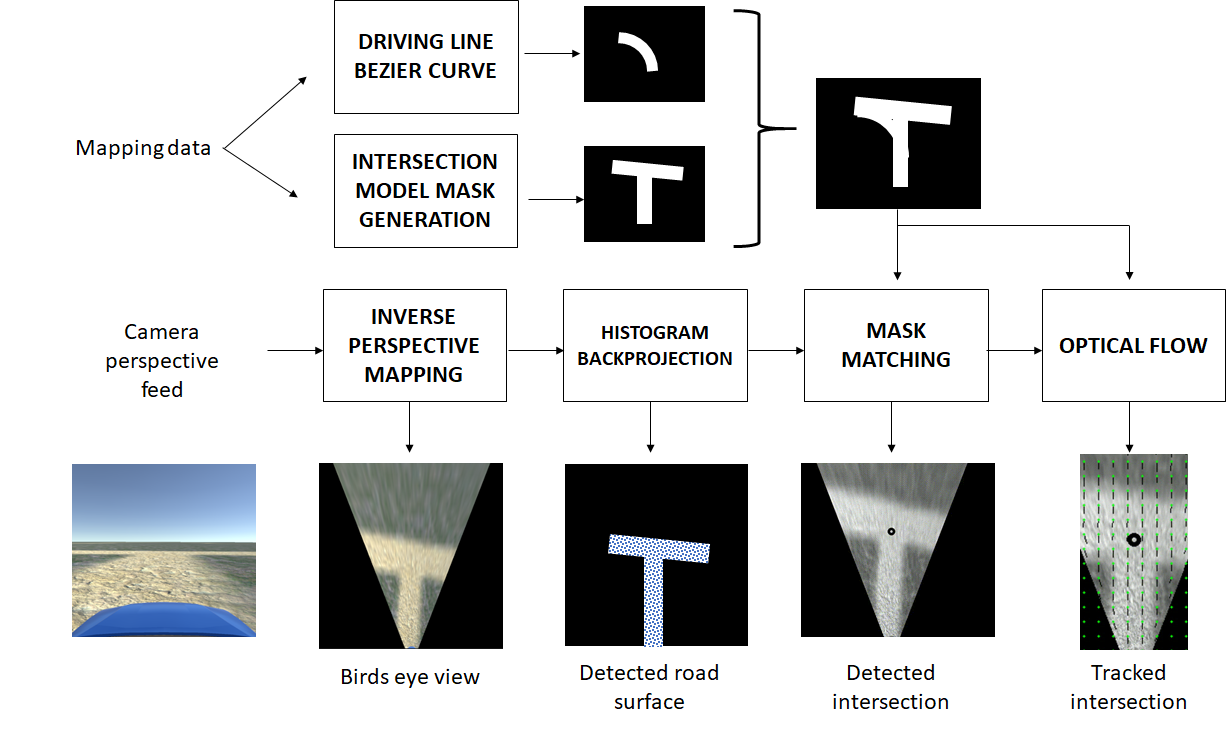
\includegraphics[width=0.95\textwidth]{systemOverview.png}
	\caption{High level overview of system stages, inputs and outputs.}
	\label{f:systemOverview}
\end{figure}


In general, the system uses inverse perspective mapping to develop a `top down' projection from the front facing vehicle camera image. \textbf{TODO: Refer to the appropriate figure for each of these steps}. An averaged histogram of local road pixels is used to develop a probabilistic road surface map using histogram backprojection. The system uses route `features' to localise the navigation goal. Route features used in the development of the system were road intersections\footnote{Examples in this paper generally consider an approach to a T junction in a custom built simulation.} however any point on a route with a clear visual pattern for the approach and exit(s) can be used. Route features are developed from mapping data (such as Open Street Map or Google Maps data) using road position nodes. A binary image mask of the upcoming route feature is developed using mapping data and is overlaid on the detected road surface. The feature is deemed detected when the proportion of feature mask covered by road surface is above a threshold. Once initially detected, the feature position is updated in subsequent video frames using a mean optical flow between frames and confirmed by remasking. A driving line through the feature can be developed and tracked by using a Bezier curve of the desired route through the feature once the initial feature model has been detected.

The discrete elements of the system with input and output as follows: 

\begin{easylist}[itemize]
	& \textbf{Road surface detection}. 
	&& \textbf{Input: }Camera feed.  \textbf{TODO: Defined data representations (F frames per second, nxm pixels x 32 bits)}
	&& \textbf{Output: }`top down' road surface map. 

	& \textbf{Route feature matching}. 
	&& \textbf{Input:} `top down' road surface map. 
	&& \textbf{Input:} Route feature generated from mapping information. 
	&& \textbf{Output: }Position in image of target route feature, if detected.
%	&& Route model mask matching
%	&& 
%	
%	&& \textbf{TODO? Explain - Inverse perspective mapping and camera lens distortion correction}
%	& Probabilistic road surface detection
%	&& \textbf{TODO? Explain - Rolling average histogram for road surface estimation}
%	& Local orientation to road edges
%	&& \textbf{TODO? Explain - Hough transform (IS THIS NEEDED?)}
%	& Route feature matching
%	&& \textbf{TODO? Explain - Matching piecewise model to detected road surface by masking}
%	& Optical flow tracking
%	&& \textbf{TODO? Explain - Using image `flow' to track feature positions for subsequent frame matching and cornering}
%	& Driving path curve matching
%	&& \textbf{TODO? Explain - Bezier curves based off feature points}
	& \textbf{Route feature tracking}. 
	&& \textbf{Input: } Previous image frame and detected location of target route feature for that frame. 
	&& \textbf{Output: }Updated location of target route feature in subsequent image frame.
\end{easylist}


\section{Related works}

Current cutting edge self driving vehicles require high fidelity 3D maps to operate effectively which are time consuming to develop and not adaptive to rapid local changes. Despite this, position localisation improvements have been achieved without high fidelity 3D mapping data using a data fusion of GPS and inertial navigation system data \citep{gpsInsFusion} correlating a detected back lane registry supported with computer vision, GPS and inertial data with map data \citep{lowCostSensorNav} and through use of Kalman filters and LIDAR in more complex environments \citep{robotLIDARSLAM}.


\citet{ipmBasedLaneDetectionApproach} also used inverse perspective mapping with k-means clustering and open uniform B-spline model for lane fitting. \citet{ipmForLaneTracking} outlined the effectiveness of Inverse Perspective Mapping for lane detection and \citet{canneyAndHoughLanes} outlined a robust lane detection approach using Canny edge detection and the Hough transform. \citet{ipmOpticalFlow} highlighted the effectiveness of inverse perspective mapping for optical flow computation, a finding that is strongly supported by the optical flow results obtained in this system.


Histogram backprojection has been used for basic \citep{histBackObjectTracking} and multi model object tracking \citep{histBackMultiObjectTrack}, \citep{histBackObjectMultiLighting}, image indexing \citep{histBackImageIndexing} and region of interest detection \citep{histBackObjectOfInterestDetection}. It has been used with sensor fusion including thermal mapping for road detection \citep{histBackThermal} and to effectively refine spatial fuzzy clustering road detection \citep{histBackRefineShadows}.

\citet{moncularLaneDetectAndTrack} outlined an approach involving the use of a Support Vector Machine to segment image road pixels from non-road pixels and an identification of road edges and control points defining the road curve. This approach is somewhat less interpretable however provides a suitable alternate and possibly more robust option for road detection. Additionally the input and output interfaces are the same as in this system which allows the option to `sub in' this approach if it is preferred. 

\citet{histogramSegmentationRoadClassification} investigated road classification from histogram based segmentation. Other road detection approaches include road surface mapping from near field driving surface models \citep{darpaChallengeRoadDetection} and matching road curvature models to detected lane boundaries \citep{intersectionDetectionSingleCamera}. Supervised convolutional neural network lane detection has had success through fully convolutional \citep{cnnLanes1} and instance segmented \citep{cnnLanes2} approaches. Spline based representation using random sample consensus for bezier splines based off road edge detection \citep{ransicBezierFit} has also shown to be effective.

\citet{modelBasedIntersection} outlined a model based recognition approached which matches intersection models to a series of road boundary points and \citet{mitLocalNavDriving} demonstrated through practical experiments that effective localisation using Open Street Map data and global waypoints is possible using a LIDAR sensor suite for local trajectory generation.




\section{Road Surface Detection}\label{s:roadSurfaceDetection}

In order to localise navigation elements a reasonable estimate of the current road surface is required. This is achieved via Inverse Perspective Mapping (IPM) and histogram backprojection. These aspects are discussed in detail in the following subsections. The road surface detection implemented is a basic road surface detection algorithm and can be outperformed by other more advanced methods. While it was suitable for developing the proof of concept system, more robust alternatives would be suggested in a live system.

\subsection{Inverse Perspective Mapping}\label{s:ipm}

\begin{figure}
	\centering
	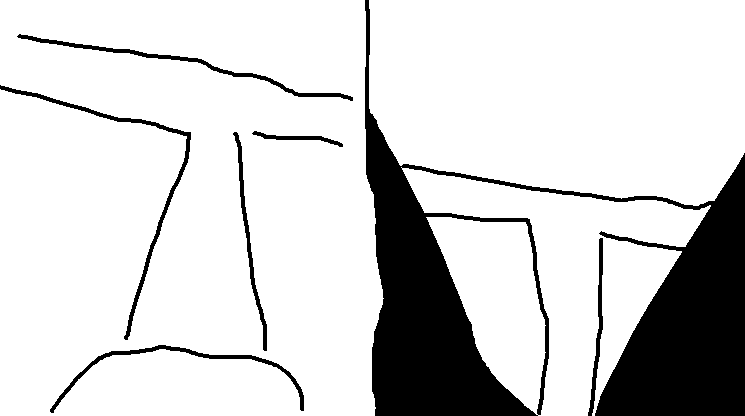
\includegraphics[width=0.95\textwidth]{RoadDetection/ipmSim.png}
	\caption{Example image from simulation (left) with IPM applied (centre) and derived IPM mask (right).}
	\label{f:ipmSim}
\end{figure}

Inverse perspective mapping (IPM) is a well established technique that involves a matrix transformation operation to remap pixels from a forward facing camera perspective to a `top down' view \citep{compVisionTextbook}. As part of this process the pixel to real world distance ratio of the inverse transformed image is determined based on known distances in the transformed image. An example of the technique applied to an image from the simulation used is included as figure \ref{f:ipmSim}. IPM assumes the perspective image is from a flat plane \citep{ipmForLaneTracking} and while road surfaces are not a flat plane, in most circumstances the local road plane can be considered approximately linear about a vehicle position as the scale of large road undulations do not generally result in significant changes locally to a vehicle. Further the system developed is robust enough to tolerate introduced error by \textbf{reasonable undulation - TODO: define (+/- x percent?)}. \citet{extendedIPM} have discussed an IPM approach that removes the flat plane assumption however it relies on a stereo camera so is out of scope for this system. This approach may prove more resilient and is worth consideration in the event a purely stereo camera based system is being developed. \textbf{TODO: Opportunity `blend' data from previous frames to estimate area outside IPM mask.}


It can be noted that the inverse perspective mapped image has a `null' area in the bottom edges where all pixels are black due to the perspective shift. This represents areas of the original perspective image that are outside the camera lens field of view. An `IPM mask' is developed which is used in later stages to ensure that any feature matching attempts are not penalised by the zero values in this area. The derived IPM mask is also included in figure \ref{f:ipmSim}. This is discussed again in section \ref{sect:route_feature_matching}. In order to correct for camera perspective as fully as possible, the camera lens effect should be corrected for \citep{fisheyeEffect} however the effects were negligible in this case and the system is robust enough that there was no requirement for this step.

\subsection{Probabilistic road surface detection}\label{s:histogramRoadDetection}

\begin{figure}
	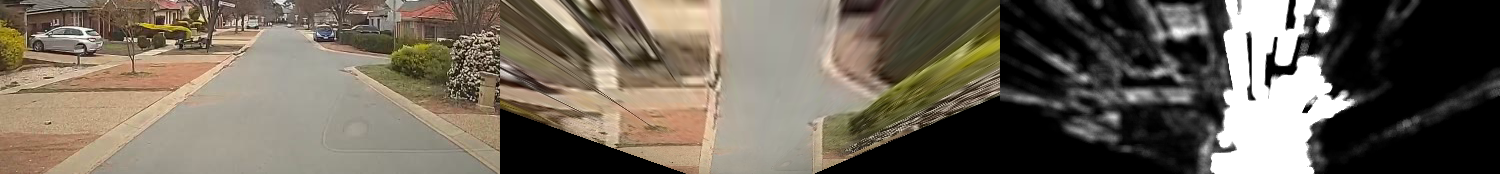
\includegraphics[width=0.99\textwidth]{RoadDetection/histRoadLive.png}
	\caption{Detected road surface from inverse perspective mapped live camera.}
	\label{f:histRoadLive}
\end{figure}

The road surface detection module uses histogram backprojection to identify likely areas of road surface. Histogram backprojection takes a provided histogram of the target, in this case the road surface, and divides it by an image histogram before convolution with a small mask to gain an estimation for the probability for each pixel in the image belonging to the target histogram \citep{histBackImageIndexing}. For this system, initially a road surface area of interest is defined, based off the near portion of road surface from the vehicle front, as indicated in figure \ref{f:histIPMcompare}. While this relies on the assumption that the vehicle starts on a road surface, it has the benefit of flexibility in detecting dynamic road surfaces. A histogram of this area is used to inform a rolling average histogram which considers the previous five frames. This is histogram is backprojected over the image to obtain a road surface probability for each pixel. An example of the detected road surface from an IPM transformed live camera feed is included as figure \ref{f:histRoadLive}. \textbf{TODO: Camera data}



While the road detection approach used for this system works with both the inverse perspective mapped image and the raw camera perspective image, in this instance it was applied after IPM transformation. It was clear from early tests that a better road surface detection was obtained when the IPM transformation occurred as the initial step \textbf{TODO: Quantify (refer to results)}. Figure \ref{f:histIPMcompare} demonstrates the significant degradation in detected surface quality when IPM transformation is applied after the road surface detection. It was also noted that when IPM was applied after road surface detection, probabilities were skewed based off pixel stretching as a result of the IPM transformation. For this reason it was determined that road surface detection should occur after IPM transformation.

\begin{figure}
	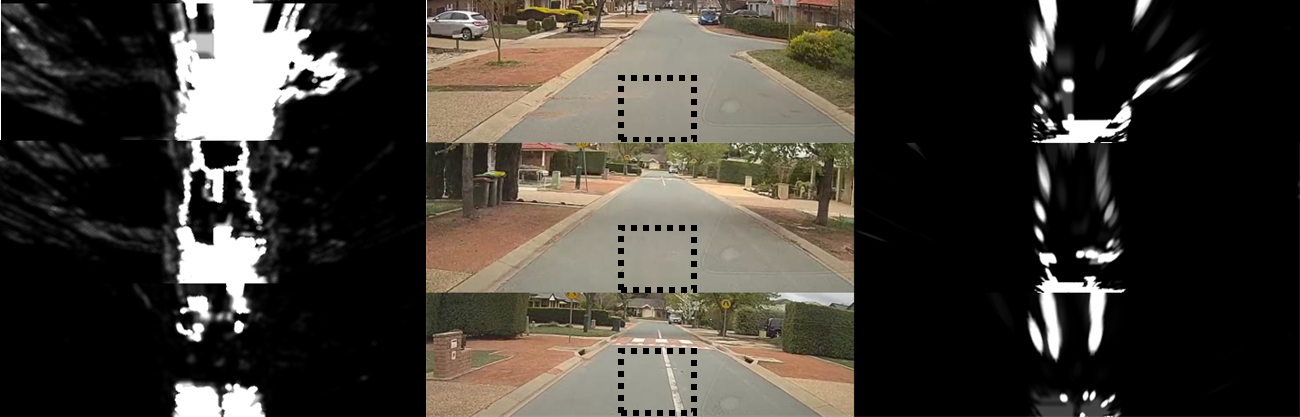
\includegraphics[width=0.99\textwidth]{RoadDetection/histIPMcompare.png}
	\caption{Comparison of histogram backprojection conducted after IPM transformation (left) and prior to IPM transformation (right). Raw image used (centre) includes indicative sampling area of interest used.}
	\label{f:histIPMcompare}
\end{figure}



%\begin{wrapfigure}{h}{0.5\textwidth} %this figure will be at the right
%	\centering
%	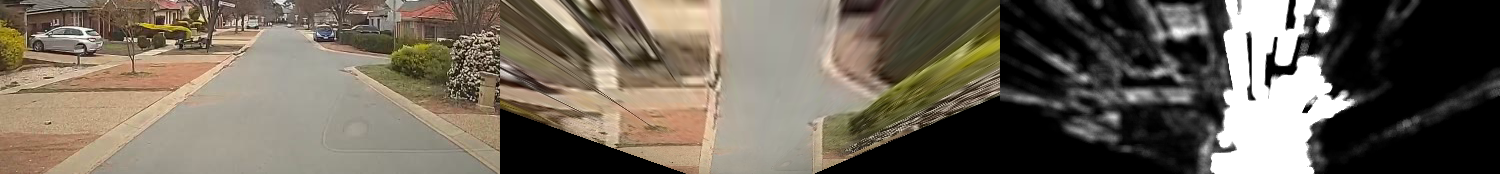
\includegraphics[width=0.5\textwidth]{RoadDetection/histRoadLive.png}
%	\caption{Detected road surface from live camera.}
%	\label{f:histRoadLive}
%\end{wrapfigure}


\citet{histBackRefineShadows} outline a shortfall with this style of road surface detection is that it can be prone to error when the road surface has little colour difference to the surrounding environment. The approach suggested in that case includes the use of thermal sensing so is not applicable for this system. If the system is required to operate in a more difficult to segment environment a more robust road detection approach may be needed. 


\section{Route Feature Matching}\label{sect:route_feature_matching}

\textbf{The system matches route `features' based on points defining relevant road segments - TODO: Expand on this for reader}. While GPS mapping data format can vary, the general common factor is that roads are defined by a series of points (nodes). These points can be used to develop a model of the road and in this case, key features. Features considered involved road intersections such as T junctions and side roads. The `main feature node' is considered to be the node central to the feature, for example the node in the middle of an intersection. A developed feature mask is used to determine if the detected road pixels match the feature. The following subsections outline the development of the route feature mask, the driving line mask and the subsequent matching process.

\subsection{Feature mask development} \label{s:maskDevelopment}

In order to develop a feature model, the feature point (node central to the intersection in this case) was placed as a starting point centrally on a blank mask. The feature mask is then developed by linearly connecting adjoining nodes. The pixel distance between nodes is defined based on the real world distance between nodes scaled using a pixel to real world distance ratio that is identified during the IPM process. It is important to note at this stage that the feature mask consists of multiple sub masks; each connection to the feature point is kept as an independent mask \footnote{Maintaining individual sub masks results in a more robust feature detection. This is discussed later in the paper.}. The width of these connections is scaled to the desired projected width for vehicle movement. An overview of the feature mask creation is included as figure \ref{f:featureMaskDevelopment} with the individual sub masks being represented by differing shading in the central sub figures. The final step in developing the feature mask is to mask it to the non-null areas of the inverse perspective mapped image. This is done using a bitwise AND operation between the developed feature mask and the IPM mask. The purpose of this step is to ensure that portions of mask features such as side roads are not considered if they fall outside the inverse projected image space. 

\begin{figure}
	\centering
	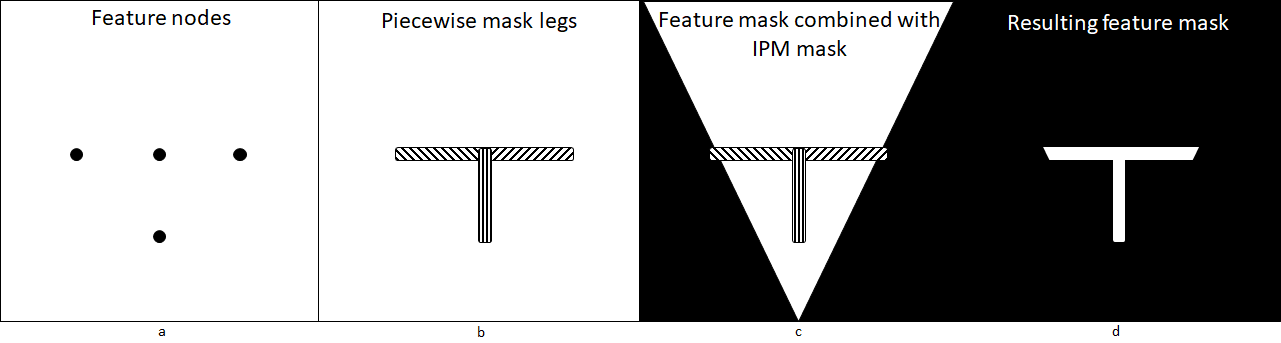
\includegraphics[width=1\textwidth]{FeatureMatching/featureMaskDevelopment.png}
	\caption{Process of developing feature mask developed feature nodes. Nodes are placed (left) and individually connected to main feature node (centre left). Shading differentiates between sub masks. The initial feature mask is then combined with the IPM mask (centre right) to obtain the final model mask (right)}
	\label{f:featureMaskDevelopment}
\end{figure}

For this system, the mask development process only considered the feature node and immediate connecting nodes. A more robust approach which considers additional approach nodes is discussed in section \ref{s:discussion}-\ref{s:improvements}.

\subsection{Driving line curve mask} \label{s:drivingPathMatching}

In order to allow a controller to effectively action system outputs there needs to be consideration given to vehicle turning arcs. This is addressed by incorporating a `driving line curve' into the mask to ensure the detected feature has room for the vehicle to turn through it. The driving line curve mask is developed using a quadratic bezier curve defined by the approach node, the feature node and the exit node. Once the driving path curve mask is developed it is masked by the IPM mask and added to the route feature masks in order to ensure the developed driving line is also on a detected road. 

The quadratic bezier is generated simply by a series of linear interpolations over the range $t=0...1$. Linearly interpolating \textit{t} between the approach node to feature node and the feature node to exit node provides two new points, \textit{p0} and \textit{p1}. Linearly interpolating \textit{t} between \textit{p0} and \textit{p1} provides a point \textbf{B(}\textit{t}\textbf{)} along the quadratic bezier curve. The full bezier curve is given by \textbf{B(}\textit{t}\textbf{)} for the range $t=0...1$. A visualisation of this is included as figure \ref{f:quadraticBezier}.

\begin{figure}
	\centering
	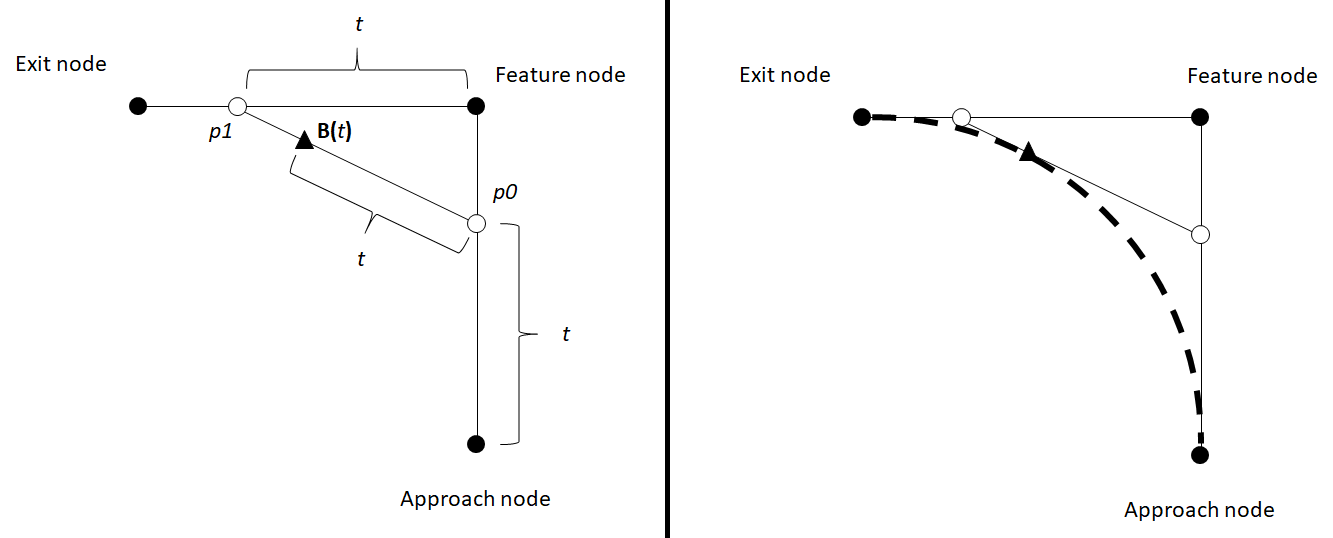
\includegraphics[width=1\textwidth]{bezier/quadraticBezier.png}
	\caption{Bezier curve interpolation: Generating \textbf{B(}\textit{t}\textbf{)} for $t\approx0.7$ (left) and the full bezier curve (right)}
	\label{f:quadraticBezier}
\end{figure}

The development of the driving line will generally need to be customised for the specific vehicle implementing this system in order to account for specific parameters such as turning circle. This is implemented by amending the approach and exit node to be a desired distance from the feature node such that a developed bezier curve represents the turning circle capability of the vehicle. 

\subsection{Feature mask matching} 

Features are considered detected based off a probability threshold; that is a feature is considered as a binary `detected' or `non-detected' based on a comparison between a defined threshold and the determined probability. Let $P(\textbf{F})$ be the probability that a feature $\textbf{F}$ is detected for a given detected road surface $\textbf{R}$ and $P(\textbf{F}_{sub,k})$ be the probability that the k'th sub feature $\textbf{F}_{sub,k}$ is detected. $P(\textbf{F}_{sub,k})$ is determined by the summation of the Hadamard product (elementwise product) between the feature sub mask and the detected road surface divided by the element sum of the feature sub mask, as outlined in equation \ref{eq:subMaskProbability}. The assessed probability that the route feature is detected is the minimum sub feature probability as per equation \ref{eq:featureProbability}. The probability threshold for $P(\textbf{F})$ is a design decision that can be amended based on factors such as noise and road surface detection output, for example considering a probabilistic or binary thresholded detected road mask. \textbf{Talk about what was explored as thresholds and consequences.}

\begin{equation}\label{eq:subMaskProbability}
	P(\textbf{F}_{sub,k}) = \frac{\sum_{i,j=1}^{n} (\textbf{R} \circ \textbf{F}_{sub,k})_{ij}}{\sum_{i,j=1}^{n} \textbf{F}_{sub,k,ij}}
\end{equation}

\begin{equation}\label{eq:featureProbability}
	P(\textbf{F}) = min\{\textbf{F}_{sub,k}:k=1,...,n\}
\end{equation}

Initial detection approaches involved using a single full feature mask as per equation \ref{eq:subMaskProbability} in lieu of sub features however this approach is significantly less robust. In the event of a noisy surface detection it is conceivable that the sum total of all road pixels under the mask may meet a generous threshold even if one element of the feature is not detected at all. Considering all elements of the feature as separate masks and using the minimum detected probability eliminates this and ensures that each feature element has a minimum detection. 

Once the feature is detected, the centre point is then the main feature node location from the initial mask. It is possible to further refine this by `bracketing' about the detected feature point by testing surrounding points. This may not be required however as assuming the vehicle is central on the road surface the midpoint of the detected feature will be aligned to the midpoint of the route feature and the inclusion of the driving line in the feature mask assures the chosen line is on the detected road surface.

\section{Route Feature Tracking}\label{s:roadFeatureTracking}

Mean optical flow was used to estimate an updated feature node location in order to track the detected route features. This was then confirmed using the masking approach discussed in section \ref{sect:route_feature_matching}. In general, optical flow options can be considered as sparse where a few key points are tracked, or dense where a large number of points up to individual pixels are tracked. It should be noted this categorisation represents ends of a continuous range rather than a binary category option. 

The Gunnar Farneb{\"a}ck method \citep{opticalFlowSolution} is a dense approach which considers a polynomial expansion to approximate pixel neighbourhood and minimises an error function for an approximated local displacement. By contrast, the Pyramidal Implementation of the Lucas Kanade Feature Tracker outlined by \citet{opticalFlowLKPyramidal} relies on key tracking points in an image. The Lucas Kanade approach was considered initially as a sparse option due to efficiency however it did not perform well. It is assessed that the random surface textures in this case lack the definition to be tracked effectively via this method. The Two Frame Estimation proposed by \citet{opticalFlowSolution} (the `Gunnar Farneb{\"a}ck method') was identified to perform better in the image frames that are typical of this problem. Similar relative performance results were identified by \citet{opticalFlowLKvsDenseUAV} when considering moving images of near grass surfaces. The Gunnar Farneb{\"a}ck method was employed to track pixels in a small region of interest on the inverse perspective mapped camera image. The region of interest is comparable to the histogram region of interest for backprojection as discussed in section \ref{s:roadSurfaceDetection}-\ref{s:histogramRoadDetection}. The smaller region of interest mitigated the use of a dense algorithm while improving mean optical flow calculation accuracy.

\begin{wrapfigure}{r}{0.5\textwidth} %this figure will be at the right
	\centering
	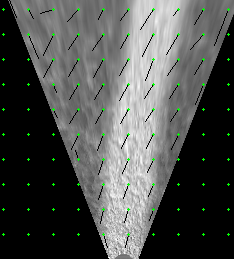
\includegraphics[width=0.5\textwidth]{FeatureTracking/optical_flow_trails.png}
	\caption{Selected optical flow lines visualised. Black tails indicate flow vector from each point.}
	\label{f:optical_flow_trails}
\end{wrapfigure}

The benefits of optical flow tracking in a smaller region of interest of the inverse perspective map are as follows:
\begin{easylist}
	& Allows effective processing of dense optical flow due to a small total number of pixels.
	& Avoids noisy areas such as extremity pixels which are warped by IPM.
	& Optical flow space occurs in the same space as the feature matching allowing a direct application of mean flow to the new estimated position.
\end{easylist}

A visual example of optical flow output for a small selection of pixels is included as figure \ref{f:optical_flow_trails}. It can be seen from this image that not all flow vectors are uniform and in particular at the edges of the mask there are large distortions. These distortions are expected due to the discontinuity and do not affect the result as the system only considers the optical flow from a range of pixels to the direct front of the vehicle. The average of these more uniform flow vectors is used to provide an effective estimate of the updated feature location. The mean optical flow approach involving a small region of interest of 100px high by 36px wide performed effectively in cases where the mean flow was in the order of 5px or less, corresponding to an approximate 5\% of the window height. \textbf{TODO: RESULTS FROM PRESENTATION.}

Once the mean optical flow has been developed, the estimated feature position is updated and the position delta is also used to update the feature model masks accordingly. Once the model masks have been updated, the IPM mask is applied and the new approximated feature position is confirmed using route feature matching as discussed in section \ref{sect:route_feature_matching}. If the new location of the approaching node places the curve defined by the driving path at the bottom of the image, the vehicle has arrived at the tracked feature and the route feature matching can generate the next route feature. In the event the feature is otherwise no longer detected, a bracketing approach can be used to attempt to relocate it.

\section{Discussion} \label{s:discussion}

\textbf{TODO: Start positively - This system as developed effectively identifies route features and driving lines through features. The system was developed and refined in simulation with verification conducted using live dashcam footage. }The system outlined in this paper does have the limitation that it is designed around a single road surface which is assumed to be fully drivable. Multi lane detection and detection and tracking of other vehicles is outside the scope of the system as developed. While a controller may manage these factors, there is no explicit consideration for non traversable road surfaces (for example a lane with opposite direction of travel) or on road obstacles. Within these specified limitations however, the system as outlined demonstrated an ability to approximate a road surface and very effectively identify and track route features and driving lines where the road surface identification was effective. The system is easy to understand at a high level, as per figure \ref{f:systemOverview} and has interpretable inputs and outputs which can be used in other aspects by both human and machine applications. This provides a system suitable for navigation localisation redundancy or alternatively in a low cost entry level setup.

\textbf{System parameters.} The system has a range of parameters to be specified which allow customisation to both vehicle and route specifications. System parameters include: 

\begin{easylist}
	& \textbf{Camera parameters.} \textbf{TODO: Expand this section for future work (appendix)}
	&& \textbf{Field of view.} The camera field of view affects the visibility of road surfaces off the direct line of travel at the close edges of the vehicle, especially after IPM is applied. If the field of view is too narrow, route features such as side streets may be lost prematurely. As such, a field of view with reasonable vision to the left and right of the driving surface in the near distance is required.	
	&& \textbf{Frame resolution.} This system remains effective at lower resolutions so the full resolution of the camera frame may not be required. While larger frames contain more detail in general the system can trade some resolution for computational time savings without significant losses. Frame resolutions used in testing varied from 512px to 150px widths. 
	&& \textbf{Frame processing frequency.} While not strictly a camera parameter, the frequency with which the system processes the frames is a key consideration and will generally relate to the processing speed of the implementation. A lower frequency of frame processing results in a higher likelihood of route feature tracking errors and less redundancy in any detection failures. Frame frequency for this test was as low as 10Hz with no noticeable degradation in feature detection or optical flow tracking. This parameter should be considered in context with resolution to ensure that optical flow tracking remains effective.
	& \textbf{Road surface detection.}
	&& \textbf{Assumed road surface region.} The histogram backprojection relies on a specifieds area in front of the vehicle to be sampled for the histogram for backprojection. This region will vary based on the physical setup of the vehicle and camera mount and should be chosen carefully to avoid introduction of additional noise such as road edges. The size of this region is dependant on the camera field of view; a narrow camera field of view will restrict the area that can be reliably sampled as road surface.
	&& \textbf{Feature detection probability threshold.} This value is considered when determining if a feature has been detected. A value of 1.0 will require each pixel of the feature mask to be over a road surface pixel with a probability of 1.0. The only occasion this is feasible is in the case the detected road surface is a purely binary thresholded mask. Realistically the detection threshold probability needs to be less than 1.0 to account for noise and uncertainty in the detected road surface.
	& \textbf{Feature development}
	&& \textbf{Image pixel to real world distance ratio.} This can be determined from the IPM procedure based on known real world distances as projected after IPM occurs. This is required for the development of route feature masks at an accurate scale. 
	&& \textbf{Route feature mask width.} The pixel width to use when developing the route feature mask. This width does not need to represent a full vehicle width as the driving line mask will ensure the vehicle can pass through the feature. In the development of this system, the route feature mask width was 25\% of the vehicle width. If this width is too great there is a risk that the combined driving line and feature mask may be wider than the feature itself, leading to a failure to detect the feature.
	&& \textbf{Driving line mask width.} Related to above however this needs to have a real world width to comfortably accommodate the vehicle width to ensure driving line through the feature will ensure the vehicle remains on the detected road surface.
\end{easylist}

These parameters directly impact the effectiveness of the system however are generally easy to tune as the entire system is human interpretable thus the effect of a parameter can be directly observed and understood.

\textbf{IPM and optical flow effectivenes.} \textbf{TODO: Does this need to be chopped? Integrated into results? other?} As noted in section \ref{s:roadSurfaceDetection}-\ref{s:ipm}, IPM transformation has the assumption of a flat plane which will not be the case along many routes. It was assessed that the local area in front of the vehicle \textbf{can be assumed to be linearised and testing demonstrated negligible affect on the localisation system TODO: why can it be assmued (+/- range) and what is the negligable affect? Quantify and refer to results? }when route undulations were incorporated. As a result it is assessed that this assumption can be held as feasible in standard driving conditions. It should also be noted that the optical flow estimation of the updated feature position was very effective in testing and once detected, features were not lost until arrival at the feature location. Regardless, as discussed in section \ref{s:roadFeatureTracking} it is important to build in redundancy and any controller implementing this system will need to include suitable actions in the event of complete feature loss.

\subsection{Performance}

\textbf{TODO: Difficulty quantifying performance}

\textbf{TODO: Key metric areas}

\subsubsection{IPM and Histogram Backprojection}

\textbf{TODO: Discuss this - range of IPM, data loss, road narrowing etc}

This is highlighted in figure \ref{f:ipmHistogramResults} which provides examples of far (100m), mid (30m) and near (15m) maximum IPM ranges for a straight and curved road. \textbf{TODO: IPM image loses road in far, some appreciation of poorer RSD}

\begin{figure}{}
	\centering
	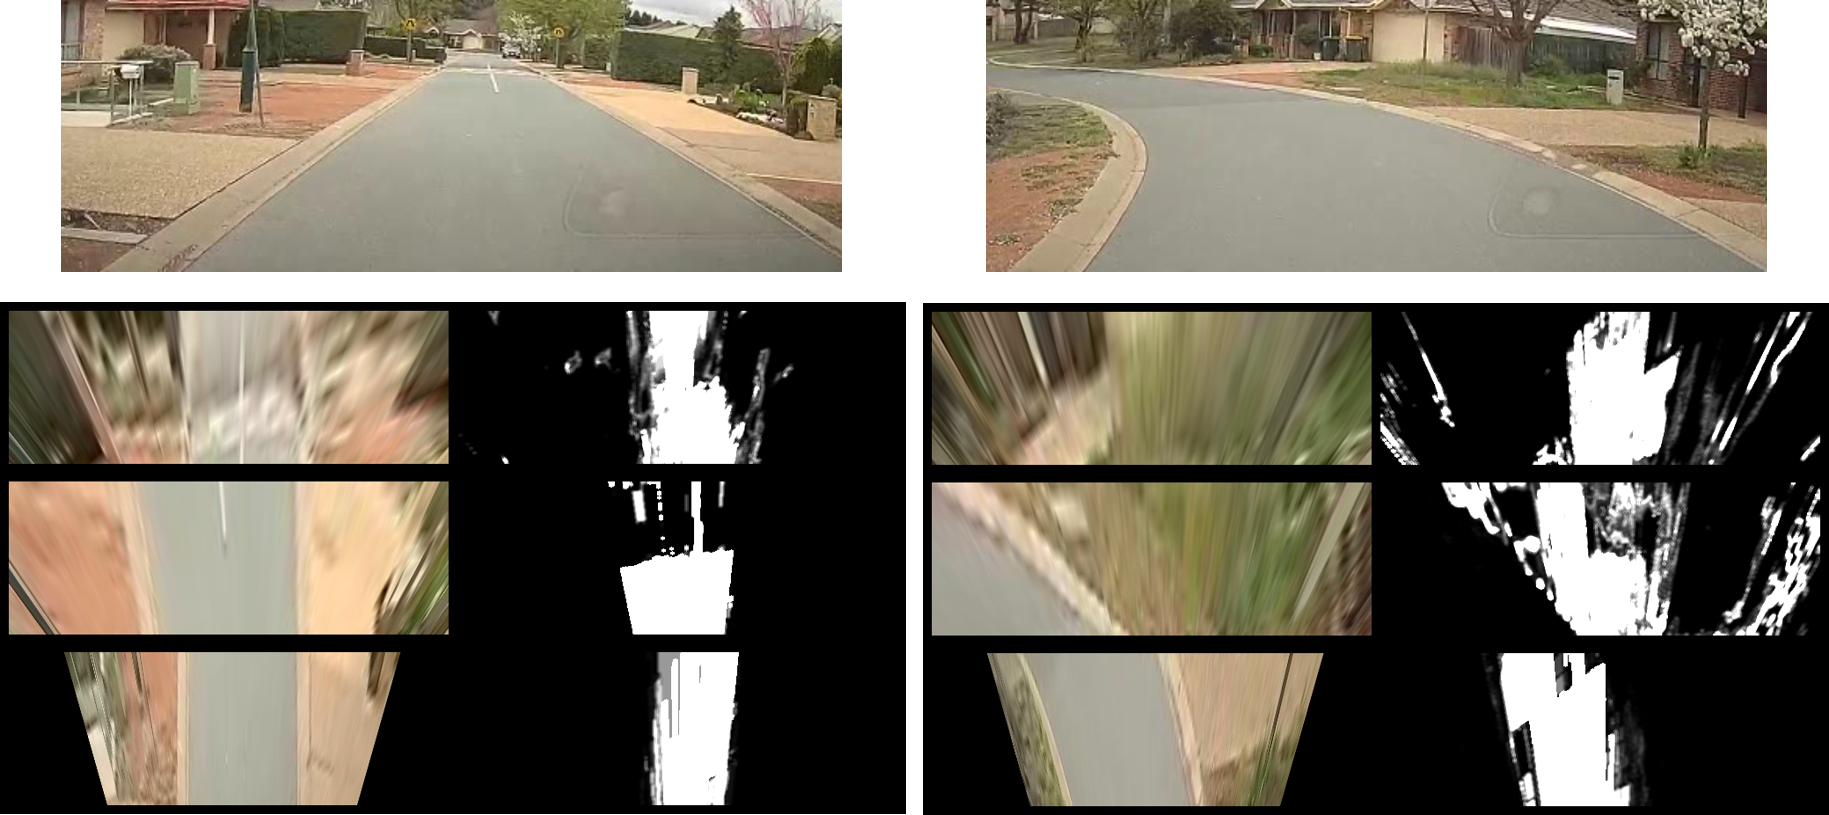
\includegraphics[width=0.99\textwidth]{Results/ipmHistogramResults.png}
	\caption{Demonstration of Histogram backprojection at far (top), mid and near (bottom) ranges for straight (left) and curved (right) road surfaces.}
	\label{f:ipmHistogramResults}
\end{figure}

An analysis of the road surface detection accuracy demonstrates clearly that the near IPM range performs more consistently and, importantly, suffers from less `false positives' where road surface is detected outside the true surface. Table \ref{t:ipmRangeRoadSurface} outlines the accuracy values in these cases \textbf{TODO: wording? Wrap it up better?}

\begin{table}[]
	\begin{tabular}{llll}
		Road type & IPM range & Correct road surface ratio & Falsely detected road surface ratio \\
		Straight  & Far       & 67.186\%                   & 1.148\%                             \\
		& Mid       & 43.761\%                   & 0.391\%                             \\
		& Near      & 74.868\%                   & 0.486\%                             \\
		Curved    & Far       & 0\%                        & 20.558\%                            \\
		& Mid       & 0\%                        & 30.798\%                            \\
		& Near      & 75.261\%                   & 0.818\%                            
	\end{tabular}
	\caption{Accuracy of detected road surface for varying IPM maximum ranges for straight and curved roads}
	\label{t:ipmRangeRoadSurface}
\end{table}

Additionally it was noted that the quality of detected road surface degraded by as much as 50\% if detection was applied prior to IPM transformation. Figure \ref{f:ipmHistorgramReverse} demonstrates the result of applying road surface detection to the perspective image and applying the IPM transformation to the detected road surface. This detection example corresponds to the `near' range detection in figure \ref{f:ipmHistogramResults} and clearly demonstrates the additional distortion to the IPM transformed road surface.


\begin{figure}{h}
	\centering
	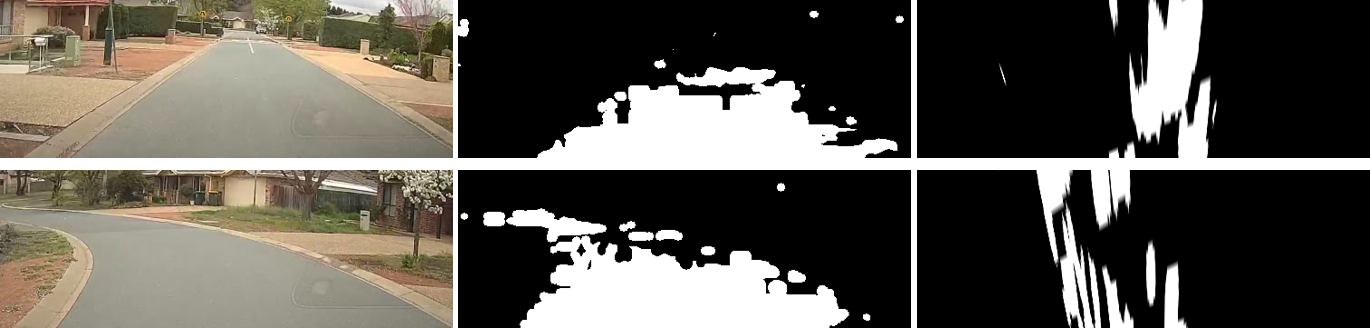
\includegraphics[width=0.99\textwidth]{Results/ipmHistorgramReverse.png}
	\caption{Road surface detection performance when applied prior to IPM transformation for roads in figure \ref{f:ipmHistogramResults}.}
	\label{f:ipmHistorgramReverse}
\end{figure}

%
%\begin{wrapfigure}{r}{0.95\textwidth} %this figure will be at the right
%	\centering
%	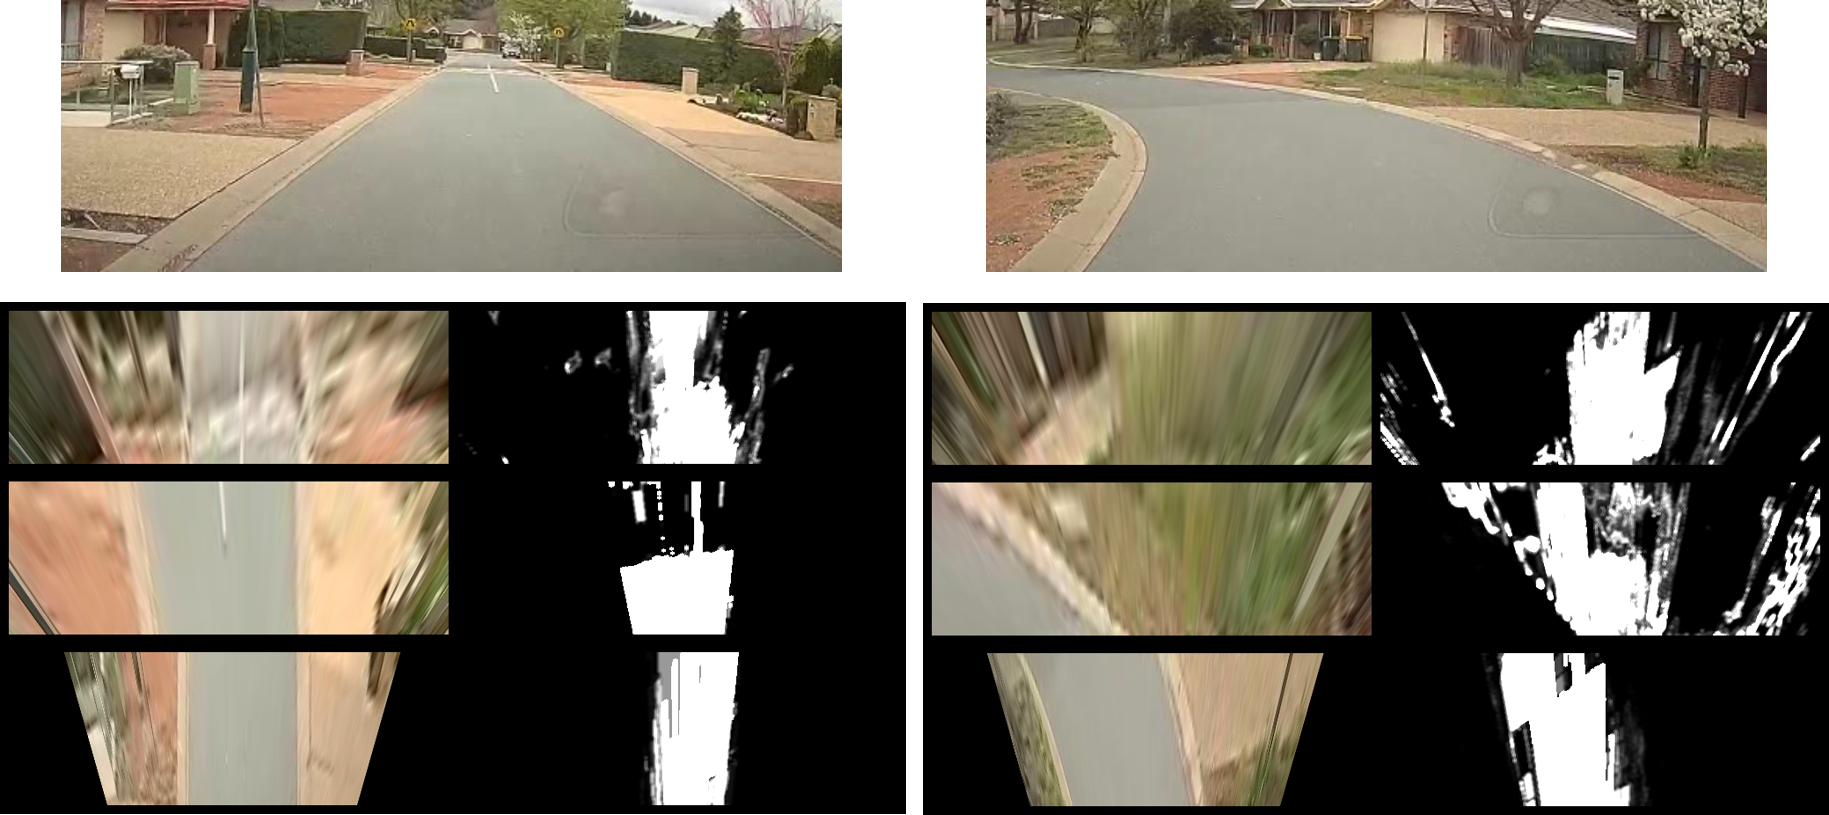
\includegraphics[width=0.95\textwidth]{Results/ipmHistogramResults.png}
%	\caption{Selected optical flow lines visualised. Black tails indicate flow vector from each point.}
%	\label{f:ipmHistogramResults}
%\end{wrapfigure}


\subsubsection{Optical Flow reliability}


\textbf{TODO: Discuss this}
As highlighted in figure \ref{f:opticalFlowResults}...
\begin{wrapfigure}{r}{0.5\textwidth} %this figure will be at the right
	\centering
	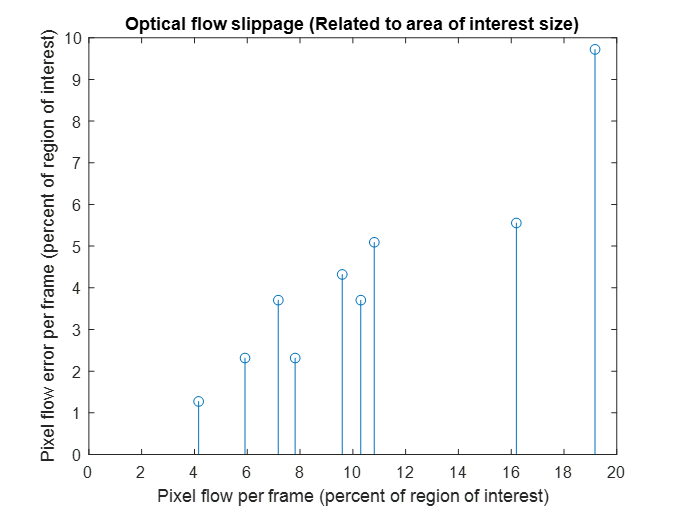
\includegraphics[width=0.5\textwidth]{Results/opticalFlowResults.png}
	\caption{Selected optical flow lines visualised. Black tails indicate flow vector from each point.}
	\label{f:opticalFlowResults}
\end{wrapfigure}


\subsection{Opportunities for future work} \label{s:improvements}

\textbf{TODO: Improved road surface detection (eg. CNN?)}

\textbf{Integration with Fuzzy Logic.} \citet{fuzzySail} present results demonstrating a very effective combination fuzzy control system for a sailing boat including the ability to tack and jibe. \citet{fuzzyGrove} outlined significant improvements in using fuzzy logic for sensor fusion and control of autonomous vehicles operating in citrus grove alleys. The system discussed in this paper involves probability based decisions throughout the process and may be a good candidate for integration with Fuzzy logic decision making and/or control.

\textbf{Known road map histograms.} The histogram backprojection uses an average histogram over the previous 5 frames. This is effective for slowly changing road surfaces however can lead to brief road surface loss when moving from one surface to another. An alternate option is to have a bank of representative road surfaces to use for the backprojection and consider the maximum probability over the range of surfaces as each pixel's probability of being a road surface. This can also be combined with the rolling average to provide a more robust assessment as well as categorise road surfaces. \textbf{TODO: Lighting effects - shade, time of day.}



\section{Concluding remarks}

\textbf{TODO: Start positively - This system does blah effectively and provides zzzz cabaility. }The resulting system has specified limitations as discussed in section \ref{sect:intro} and in particular the road surface detection approach represents a basic implementation. In addition to the societal considerations for interpretable AI, the focus on interpretable steps has the significant benefit of having a clear `plug and play' interface with other systems. As a result, when an improved road surface detection algorithm is identified it can easily be integrated to the system in place of the existing element. 

As developed, the system effectively identifies and tracks route features and provides a driving line through the identified feature. The model mask approach of feature detection provided effective feature matching in non ideal conditions and the bezier curve driving line provides a control system a constant steering angle for feature traversal. In particular the use of optical flow for route feature tracking was highly effective. 

Redundancy in autonomous systems is a critical consideration and should be included as part of any system design. A system such as the one proposed in this paper provides a low barrier to entry for simple vehicular navigation automation tasks and offers a final redundancy option in the event that a `high end' autonomous system suffers a significant sensor suite failure.


\section*{Appendices}
\ref{app:implementationDiscussion} - Implementation Discussion \\

\newpage

%
%\subsubsection{Bezier curve theory}
%\textbf{TODO: ADD THIS AS APPENDIX??!?}
%A Bezier curve is a parametric curve defined by a series of control points with the position on the curve defined by a variable $t$ ranging between 0 and 1, corresponding to the start and the end of the curve. Quadratic Bezier curves consist of three control points ($p_0$, $p_1$ and $p_2$) resulting in a quadratic equation with respect to the variable $t$. \textbf{TODO: Keep going}
%
%\textbf{TODO: IS THIS MID POINT INTERPOLATION REQUIRED? OR DOES SETTING `IDEAL' CONTROL POINTS FIX IT?}
%The formula for the basic Quadratic Bezier curve is outlined as equation \ref{eq:quadratic_bezier}. This will result in a curve as per the curve in figure \ref{fig:quadratic_bezier_simple}. A shortfall with this approach is it will result in `cutting' of the corner as the point $p_1$ is the center point of the feature. This can be addressed by \hl{using what was $p_1$ as the central point $p_c$ to calculate a middle control point to force the curve through this point}. If a constraint is added that $\textbf{B}(t)=p_c$ for some value of $t$, it is then possible to solve for the required $p_1$ to fit this constraint. The free parameter in this instance is the value of $t$ where the curve passes through $p_c$. Setting $t=0.5$ and solving for $p_c$ will set the curve to pass through $p_c$ at the mid point which was deemed suitable in this instance. The equation to force the $p_c$ constraint is included as equation \ref{eq:quadratic_bezier_constraint} and the result of forcing the constraint  $\textbf{B}(0.5)=p_c$ is visualised in figure \ref{fig:quadratic_bezier_center_point}.
%
%
%\begin{figure}[!tbp]
%	\centering
%	\begin{minipage}[b]{0.4\textwidth}
%		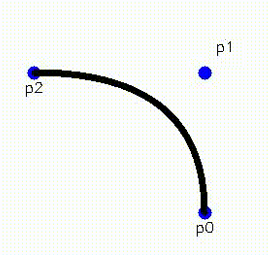
\includegraphics[width=\textwidth]{bezier/quadratic_bezier_curve.png}
%		\caption{Quadratic Bezier curve from control points ($p_0$, $p_1$ and $p_2$)}
%		\label{fig:quadratic_bezier_simple}
%	\end{minipage}
%	\hfill
%	\begin{minipage}[b]{0.45\textwidth}
%		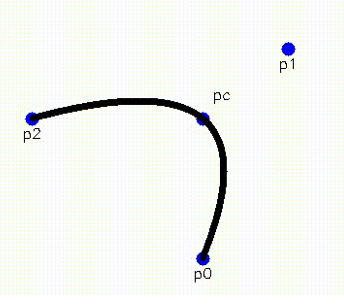
\includegraphics[width=\textwidth]{bezier/quadratic_bezier_curve_central_point.png}
%		\caption{Quadratic Bezier curve from control points ($p_0$, $p_1$ and $p_2$) constrained to pass through $p_c$}
%		\label{fig:quadratic_bezier_center_point}
%	\end{minipage}
%\end{figure}
%
%
%\begin{align}
%\textbf{B}(t) &= (1-t)^2p_0 + 2t(1-t)p_1 + t^2p_2 \label{eq:quadratic_bezier} \\
%p_1 &= (p_c - (1-t)^2p_0 - t^2p_2)/(2t(1-t)) \label{eq:quadratic_bezier_constraint} \\
%p_{mid} &= (1-a)p_1 + ap_c \label{eq:interpolated_p1}
%\end{align}
%
%It is clear the developed both path curves in both figures \ref{fig:quadratic_bezier_simple} and \ref{fig:quadratic_bezier_center_point} are not an ideal solution. As a result the final approach was to use a weighted interpolation between $p_c$ and $p_1$ where $a$ is a weighting between 0 and 1 for $p_c$ as the middle control point position; when $a=0$, $p_c$ will have full weighting over the calculated $p_1$ as the middle control point. \textbf{TODO: a = 0.5}
%


%\begin{wrapfigure}{R}{0.5\textwidth} %this figure will be at the right
%	\centering
%	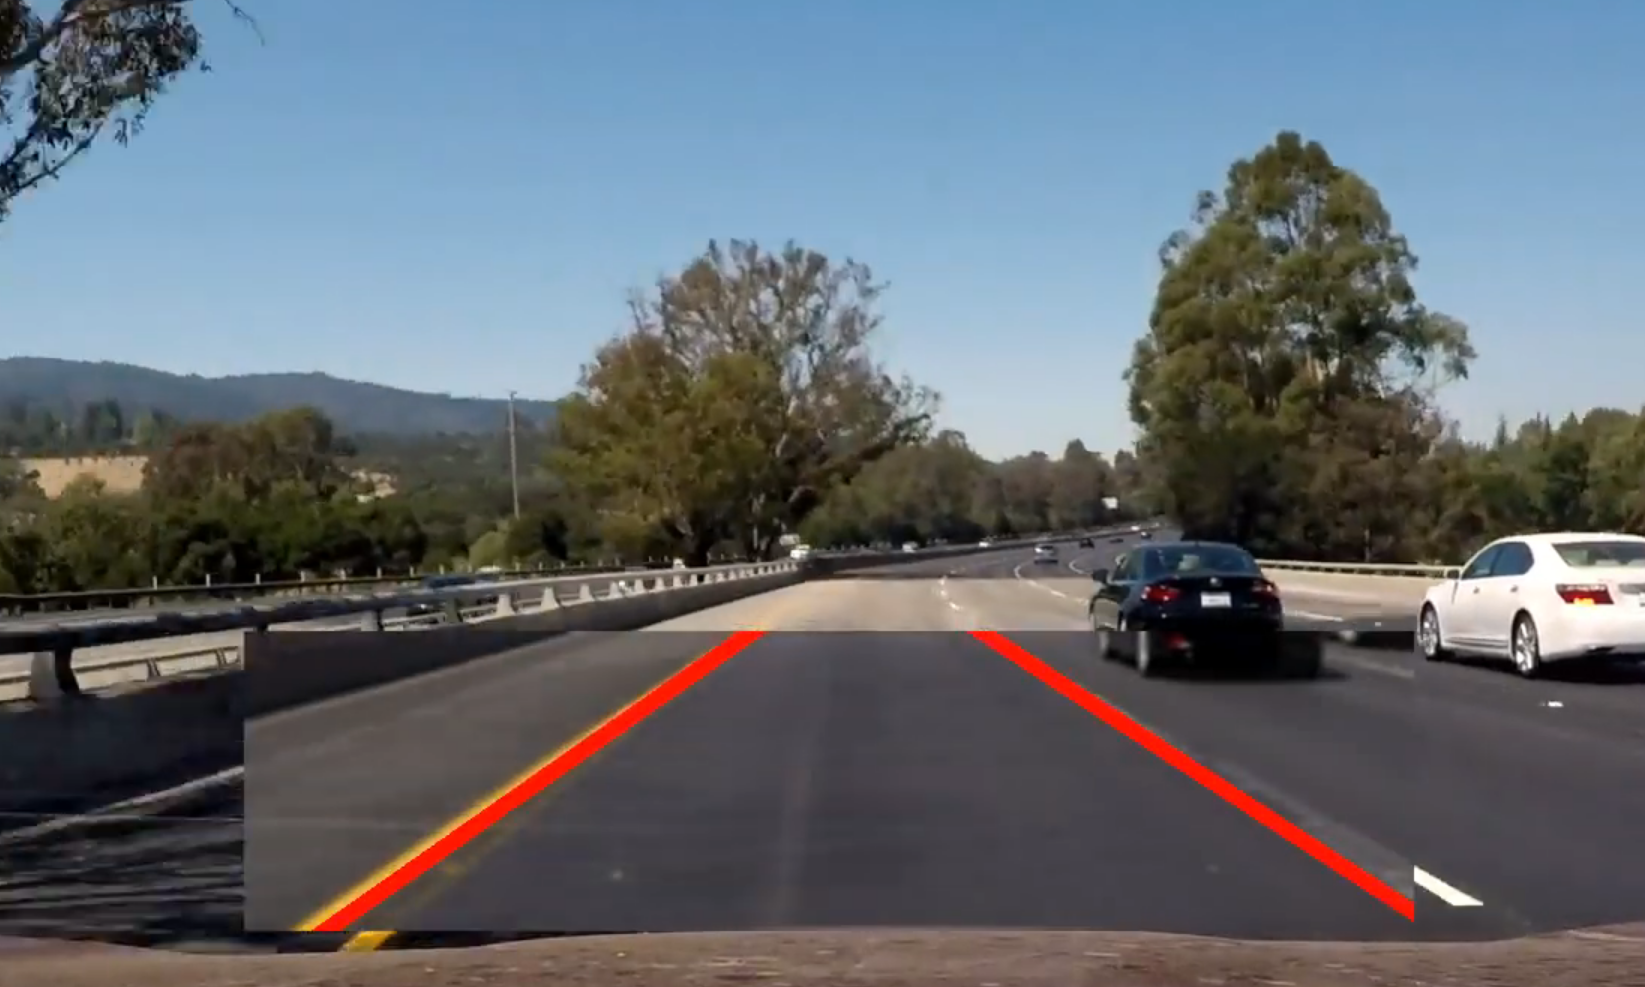
\includegraphics[width=0.5\textwidth, height=0.5\textwidth]{early_lane_detection_experiment.png}
%	\caption{Still from video feed lane detection experiment. Lower area of interest where frames are averaged visible in the bottom central part of the image}
%	\label{f:simpleLaneDetectionHough}
%\end{wrapfigure}


%\section{Current work}\label{s:currentWork}
%
%The bulk of the initial effort has been developing technical competency within informing disciplines. This includes both the CV technical competency development and addressing the simulation technical risks. This completed work is tracked in the Gantt chart in appendix REMOVED. Additionally to these aspects, familiarity projects were conducted on neural networks to consolidate the basic theory for potential future use. These `toy' projects consisted of developing neuroevolution based solutions for both a physics based ball balancing challenge over the duration of 5 minutes and custom cloned version of the mobile game `flappy bird'. Both solutions used a simple feedforward neural network coded in C\# without the use of any existing libraries with the networks evolving using a custom built genetic algorithm. The CV and simulation aspects are discussed in more detail in the following subsections. 
%
%\subsection{Computer Vision}\label{s:currentWork_CV}
%
%Before any effective computer vision approaches can be implemented a robust base of understanding of DIP is required. In order to develop a robust understanding of DIP concepts study was undertaken using a range of publicly available resources. The main resource used for structured learning was the Spring 2015 offering of ECSE-4540 at Rensselaer Polytechnic Institute in New York by Rich Radke which has the full set of recorded lectures freely available online. Basic algorithms were implemented from first principles in MATLAB which reinforced the internalisation of the concepts. More advanced computer vision concepts were subsequently researched and tested within Python using OpenCV functionality which is discussed further in this section. 
%
%The Hough Transform was used to detect straight lanes with varying levels of success. The Hough Transform converts a global detection problem into a local peak detection problem in a parameter space \citep{surveyOfHT} where straight lines in an image can be represented by a single point in Hough space \citep{houghPaper}. A brief overview of simple lane detection as a conceptual primer for the interested reader, including a discussion on the Hough transform, is included as appendix REMOVED
%
%\begin{wrapfigure}{R}{0.5\textwidth} %this figure will be at the right
%	\centering
%	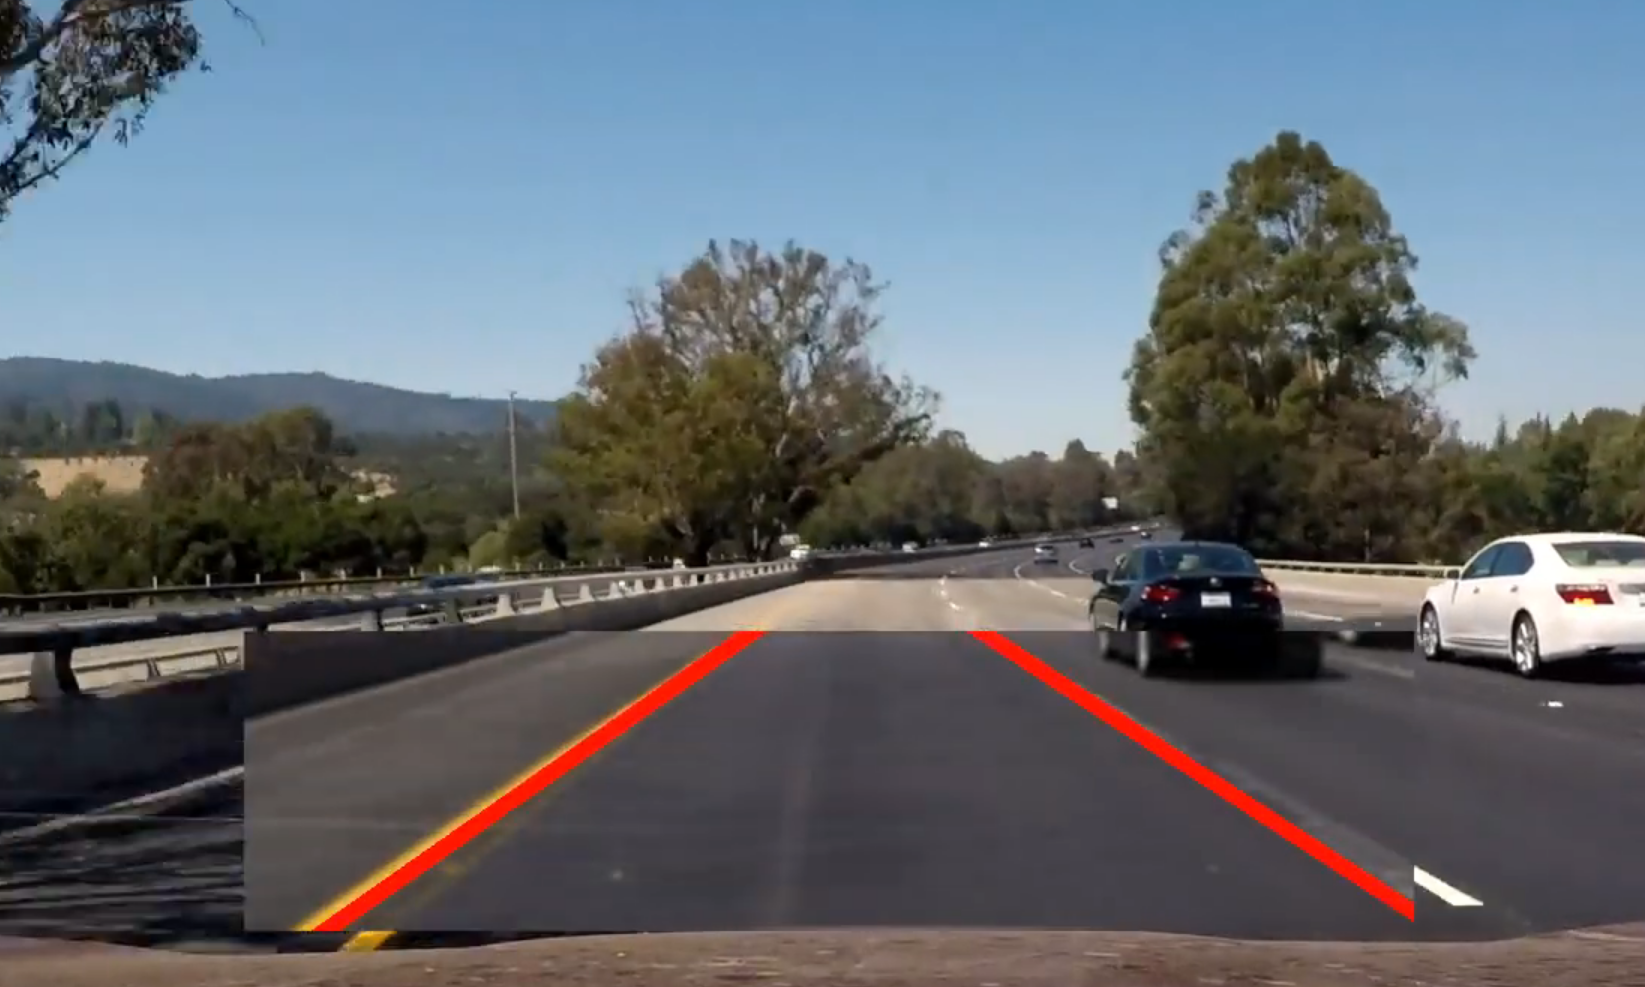
\includegraphics[width=0.5\textwidth, height=0.5\textwidth]{early_lane_detection_experiment.png}
%	\caption{Still from video feed lane detection experiment. Lower area of interest where frames are averaged visible in the bottom central part of the image}
%	\label{f:simpleLaneDetectionHough}
%\end{wrapfigure}


%
%It was noted that the simple approaches suffered when the dashed lane line was faint in comparison with other linear features and when the road was cast in intermittent shadow. The final experiment to improve on detection involved lane detection on a video feed using a rolling average of a lower area of interest of the most recent 5 frames of video as input to the lane detection for each frame. The lane detection approach involved identifying straight lines using the Hough Transform of the Canny edge detected area of interest after a low pass filter had been applied. The Hough lines were then chosen based on strength with the strongest line for each angle (side of the lane) chosen. The output consisted of the averaged area of interest with the detected lane lines in red overlayed onto the original frame. An example frame from the video output is included as figure \ref{f:simpleLaneDetectionHough}. 
%
%In order to identify the true shape of the road, more advanced techniques are required. Inverse perspective mapping is `a geometrical transform that attempts to remove the perspective effect present in an image captured by a camera pitched down towards a road' \citep{intersectionDetectionSingleCamera}, allowing a birds eye view of the scene by weighing each pixel according to its information content \citep{stereoIPM}. Inverse perspective mapping has many uses within the autonomous driving realm including vanishing point detection  \citep{ipmVanishingPoint}, attitude noise reduction \citep{ipmAttitudeNoise}, distance determination \citep{ipmDistanceDetermination}, regularizing optical flow \citep{ipmOpticalFlow}, improving relative velocity determination \citep{ipmOpticalFlowSpeed} and detailed depth information in stereo \citep{stereoIPM}. Importantly though, inverse perspective mapping is a key part in effective lane and obstacle detection \citep{ipmOpticalFlow} \citep{ipmDistanceDetermination} \citep{ipmBasedLaneDetectionApproach} \citep{ipmVanishingPoint}.
%
%The basic approach to lane detection using CV then involves correcting the image for camera lenses before inverse perspective mapping to get a `birds eye view' of the road. From this top down perspective, road/lane analysis can be conducted properly. An inverse perspective mapping calibration for the simulation was developed using the IPC implementation discussed in section \ref{s:currentWork}-\ref{s:simSystem}-\ref{s:IPC}. This calibration consists of still image of a checkerboard pattern on the horizontal plane within the simulation taken from the perspective of the camera. Corners of the checkerboard are manually identified in pixel space and the inverse perspective matrix is calculated based on the current old (perspective) and desired new (inverse perspective) positions. Automated identification of checkerboard corners is possible however the simulation camera rotation with reference to the horizontal plane is fixed therefore only a single calibration is required. The input and output of the inverse perspective mapping calibration undertaken is included as figure \ref{f:inverse_perspective_calibration}. Key considerations within the Computer Vision implementation decision process are in the following subsections.
%
%\begin{figure}[htb]% order of placement preference: here, top, bottom
%	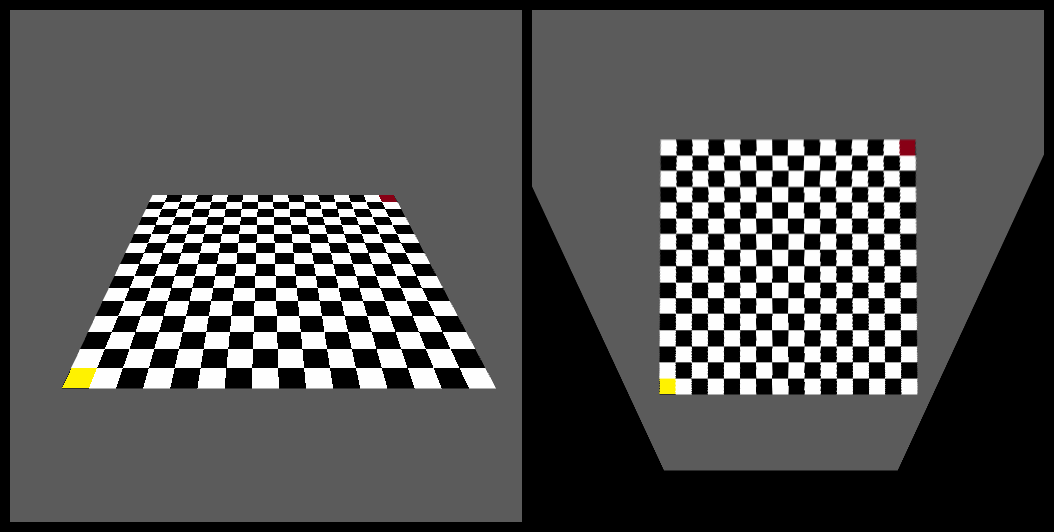
\includegraphics{InversePerspectiveEg.png}
%	\caption{Inverse perspective mapping calibration. Original camera feed \textit{(left)} and inverse perspective mapped image \textit{(right)}}
%	\label{f:inverse_perspective_calibration}
%\end{figure}
%
%\subsubsection{Use of OpenCV}\label{s:openCV}
%
%The DIP theory that was undertaken opened up the possibility to implement the CV functionality from first principles, indeed basic tools such as filtering had already been implemented in MATLAB experiments. The alternative option considered was to use an open source computer vision library called OpenCV. OpenCV has C++, Python, Java and MATLAB interfaces and is widely used in commercial applications in companies such as Google, IBM and Honda \citep{opencvWebsite}. While implementing all functions manually has merit for further reinforcement of the basic principles, the decision was made to use the OpenCV library. Rationale for this includes the following: 
%
%\begin{easylist}[itemize]
%	& Efficient high performance vectorised implementations of CV algorithms.
%	& Allows a greater proportion of time to be spent on solving the problem as opposed to implementing known algorithms.
%	& Increase familiarity with industry level tools for future use.
%\end{easylist}
%
%\subsubsection{Language choice} \label{s:pythonVc}
%
%Given the choice of OpenCV for the CV framework the options considered for the core language were C++ or Python. C++ has the advantage of being `lower level' however the OpenCV Python interface compiles down to the same C++ code so the only performance gains would be in the general program code as opposed to the CV implementations. Simulation engine considerations also played a part, as discussed in section \ref{s:currentWork}-\ref{s:simSystem}-\ref{s:simEngineChoice}, Unreal Engine uses C++ which would allow simulation code to talk directly to the OpenCV interface.
%
%Despite the above advantages, C++ comes with an increased complexity and any speed gains require a robust understanding (and implementation) of memory management. By contrast, Python presents a lower barrier to entry while maintaining the OpenCV C++ vectorised optimisation. In addition, libraries such as numpy within Python present additional highly optimised operations for array data manipulation. The decision to use Unity for the simulation engine, as discussed in section \ref{s:currentWork}-\ref{s:simSystem}-\ref{s:simEngineChoice}, removed the major benefit of C++, being the potential for the simulation code to talk directly to OpenCV, thus Python was determined to be the preferred language.
%
%\subsection{Simulation system}\label{s:simSystem}
%
%A significant element of the project deliverable is the development of the simulation system to provide sensor outputs. The intent of the simulation is to provide a pipeline of sensor feeds and potentially an interface to control a simulated vehicle based off the processed sensor data. The scope of the simulation is discussed in section \ref{sect:intro}-\ref{s:scope} with key elements of the simulation system discussed in the following subsections.
%
%
%\subsubsection{Simulation engine} \label{s:simEngineChoice}
%
%Two courses of action were available for the implementation of the simulation engine; development of a full custom simulation engine or implement simulation logic within an existing game engine. For the existing game engine option, Unreal and Unity were both considered. A full custom engine allows fine grain control over the implementation the specific requirements of the simulation however has significant overheads including the implementation of 3D visuals including rendering, texturing and importing of 3D models. It was determined that this represented a very large time commitment for negligible benefit.
%
%Both Unity and Unreal are professional 3D engines used in commercial games and computer graphics applications. They are well established and have a robust set of supporting tools. Specific considerations for each engine are as follows:
%
%\begin{easylist}[itemize]
%	& Unity:
%	&& Personal experience with workflow and language (C\#). Comfortable implementing desired features.
%	&& No C\# interface with OpenCV therefore requirement for IPC to be developed between the OpenCV processing implementation and the simulation engine.
%	& Unreal:
%	&& New, unfamiliar workflow.
%	&& Lack of familiarity and comfort with C++ which is used for scripting within the engine. `Blueprint' system does allow a visual programming approach although that represents an additional competency to be developed.
%	&& C++ code allows direct interface with OpenCV.
%\end{easylist}
%
%When considering the above factors and the OpenCV considerations discussed in section \ref{s:currentWork}-\ref{s:currentWork_CV}-\ref{s:openCV}, Unity was chosen due to the ability to `hit the ground running' based on workflow and language familiarity. It was noted that this accepts a large technical risk of IPC implementation however it was deemed to be the preferred option.
%
%\subsubsection{Interprocess Communication (IPC)} \label{s:IPC}
%
%One of the main issues identified with using Python Open CV and the Unity game engine is the ability for simulation data, for example video feeds, to be transferred from Unity to the Python process. This was assessed as a significant technical challenge and is the single largest time budgeted feature in the initial simulation work. The motivation for fast IPC was to allow real time processing of the simulation data in order to allow for potential control feedback to the simulation. Transferring image data represents a large amount of memory thus has a significant time complexity per simulation `tick'. 
%
%The initial research approach involved investigating options such as static memory buffers, shared memory and memory mapped files which would allow direct memory access to data. These options added another level of complexity and it was determined that a lower technical risk solution was to use TCP via the ZeroMQ middleware. ZeroMQ is a communications interface with implementations for both C\# and Python and is well optimised for speed.
%
% The use of this approach potentially results in slower than real time simulation processing which was mitigated by dynamic simulation time dilation, discussed in section \ref{sect:timedilation}. This approach allows easy and reliable two way communication which is required for effective feedback between the processes. This solution also offers the ability to expand off a single local machine, for example a hosted simulation with remote processing. While this is well out of scope of this research it presents additional flexibility for future development.
%
%Once the IPC approach was confirmed, the data handling pipeline between the Unity (C\#) and Python processes was developed. The final simulation output data structure for video feed is a flattened 3D byte array with four bytes for each $(x,y)$ pixel coordinate, representing the Red, Blue, Green and Alpha image colour channels. The Python process casts the byte stream as a byte array and reshapes the data to a 3D array. The fourth element of each colour value (the Alpha channel) is redundant and is removed. This results in a final data structure consisting of a 2D array of 3 element vectors of bytes which is the required data structure for OpenCV processing operations. 
%
%\subsubsection{Simulation time dilation}\label{sect:timedilation}
%
%There is a requirement to implement dynamic time scaling in the simulation order to maintain time synchronisation with the external process. The simulation scales time based on the desired processing update rate and the real time that the IPC process and external data processing takes. This allows simulation complexity scaling without the danger of temporal desynchronisation between simulation and external processes.
%
%The implementation of time dilation involved a simulation controller that runs the simulation for a set time based off the desired sensor processing rate. After this time has elapsed, sensor data is collated and sent to the external processing program via the IPC process outlined above and the simulation pauses. On completion of the data processing, the external program sends an acknowledgement in return which triggers the next simulation tick. This has been implemented and was initially tested by sleeping the processing thread for several seconds each tick. Time dilation with IPC was also tested using an initial prototype of the simulation; two stills from this test from the Python process output video showing the raw feed and the canny edges is included as figure \ref{f:simPrototypeIPCTest}.
%
%\begin{figure}[htb]% order of placement preference: here, top, bottom
% 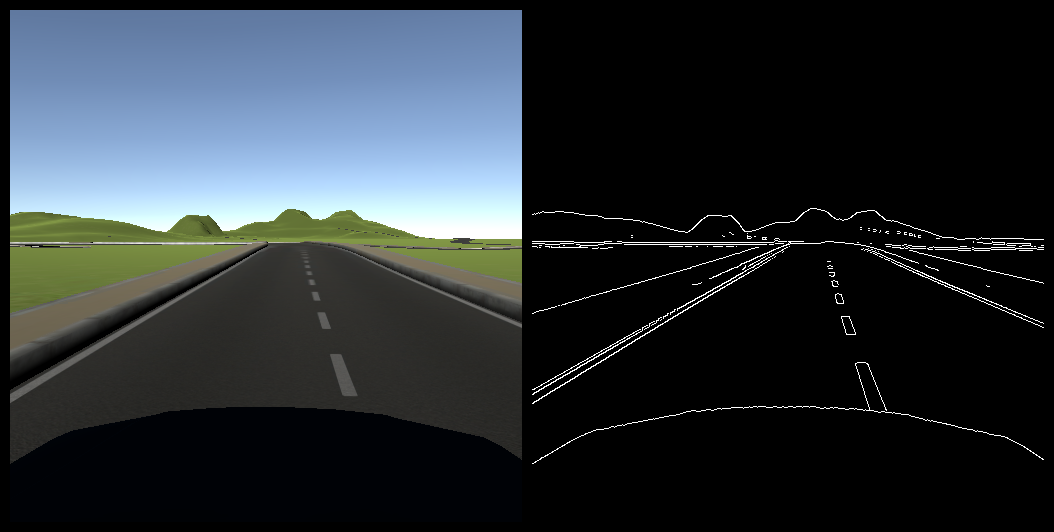
\includegraphics{simPrototypeIPC.png}
% \caption{Still from video feed of simulation prototype test. Original camera feed \textit{(left)} and canny edges of feed \textit{(right)}}
% \label{f:simPrototypeIPCTest}
%\end{figure}
%
%\section{Future work}
%
%
%\subsection{Computer Vision}
%
%\subsubsection{Lane detection}
%
%Detection of straight lane lines has been completed in the familiarisation activities conducted as discussed in section \ref{s:currentWork}-\ref{s:currentWork_CV} and demonstrated in figure \ref{f:simpleLaneDetectionHough}. Alternative approaches to lane detection which may be considered include k-means clustering \citep{ipmBasedLaneDetectionApproach}, road classification from histogram based segmentation \citep{histogramSegmentationRoadClassification}, road surface mapping from near field driving surface models \citep{darpaChallengeRoadDetection}, matching road curvature models to detected lane boundaries \citep{intersectionDetectionSingleCamera} and open uniform B-spline model lane fitting \citep{ipmBasedLaneDetectionApproach}.
%
%A more complex challenge is identifying a curved lane. Supervised convolutional neural network lane detection has had success through fully convolutional \citep{cnnLanes1} and instance segmented \citep{cnnLanes2} approaches. Spline based representation using random sample consensus for bezier splines based off road edge detection \citep{ransicBezierFit} has also shown to be effective. The current planned approach is lane edge detection via polynomial fitting of edge pixels detected by sliding window. An overview of the current implementation plan for the sliding window detection approach is included as appendix REMOVED. The technical risk of this aspect is low to medium.
%
%
%\subsubsection{Intersection detection}
%
%Intersection detection presents a more challenging prospect than simple lane detection. The simplifying assumption of a single left and right lane edge is removed when intersections are introduced. The SCARF (Supervised Classification Applied to Road Following) approach of using Gaussian colour models to identify road surface before road model matching \citep{scarf} and UNSCARF (UnSupervised Classification Applied to Road Following) approach using feature identification, clustering and edge detection and road model matching \citep{unscarf} have both demonstrated an ability to detect lanes and intersections in non ideal conditions using a dual camera setup, although not in real time \citep{scarfAndUnscarfPresented}. A data driven model using a `virtual camera' supported by model based intersection matching has also shown promise \citep{alvinnVC} however this requires prior information to reconstruct virtual images. Alternatively, once a binary road surface map is obtained, row based histograms can be used to identify intersection locations by interpolation between intersection models \citep{intersectionDetectionSingleCamera}.
%
%One example of effective intersection detection determined to be more directly applicable to this project is model based recognition which matches intersection models to a series of road boundary points \citep{modelBasedIntersection}. An alternate approach is using skeletonisation of the road binary mask. When the full road surface is represented by a binary mask, skeletonisation will reduce each road to a single pixel line. This road skeleton can be matched to the model skeletons. The current intent is to use edge detection to determine boundary points with the intersection model being built reasonably simply using the OSM map data. The technical risk of this aspect is medium.
%
%
%\subsection{Navigation localisation}
%
%The final step involves correlating the GPS positional data, features from video sensor feed and the navigation data to localise the navigation data to the vehicle position. Static route map matching at its most trivial relates a GPS position to the nearest point on a polyline. It is anticipated that this will be the first step in the localisation to approximate the position on the navigation route. 
%
%A LiDAR-based local trajectory generation has demonstrated through practical experiments that effective localisation using OSM data and global waypoints is possible using a LIDAR sensor suite \cite{mitLocalNavDriving}. General curve or spline matching options will be investigated and it has been identified that Markov and extended Kalman filter localisation techniques may also assist in this problem \citep{probabalisticRobotics}. The most likely solution will be a combination of the above and the model based recognition outlined by \citet{modelBasedIntersection}. The technical risk of this aspect is medium.
%
%\subsection{Simulation}
%
%The simulation development will follow the agile development process and deliver incremental feature additions and improvements. The basic features which are high priority for the early sprints are the implementation of the functionality required for the minimum viable product; the vehicle controller, the road network and the GPS sensor and navigation implementations. These aspects, as well as candidate functionality extensions are discussed in more detail in the coming subsections.
%
%\subsubsection{Vehicle controller}
%
%The vehicle controller will be implemented using the built in physics components within the Unity engine. The basic vehicle setup will consist of steering, accelerating and braking functions with vehicle movement simulated by the physics engine. An autopilot function that will follow defined waypoints from the navigation system discussed in section \ref{s:gpsNavSim} will also be developed. It is important to note that this autopilot is not based on the external analysis of sensor input but will use the exact game data. The intent of this functionality is to provide a constant video feed of a driving vehicle by a simulated driver agent for analysis and should not be confused with the autonomy solution to the main problem this research is investigating. Features such as engine power simulation will not be implemented in the initial stages but may be introduced as future features. The technical risk of this aspect is very low.
%
%\subsubsection{Road network}
%
%The road network is being implemented using a commercial tool called Easyroads 3D. This tool assists in mesh generation, placement, connection and texturing of roads as well as terrain moulding. Additionally the tool can accept map data exported from OSM. While each of these functions can be custom built individually it represents a significant time commitment and is unrelated to the core simulation. The road visible in the raw video feed of the IPC prototype test in figure \ref{f:simPrototypeIPCTest} demonstrates the implementation of a test road in Unity. The initial implementation of the road network will be simple single lane tracks. The technical risk of this aspect is low.
%
%\subsubsection{GPS sensor}
%
%The GPS sensor implementation is a simple function and required for the base sensor data analysis. The functionality will use the in engine coordinates for the GPS coordinates, as will all other data and sensors. An initial customisable random position offset will be used to simulate GPS positional error however additional functionality improvements may include a higher fidelity simulation of GPS error. The technical risk of this aspect is negligible.
%
%\subsubsection{GPS navigation}\label{s:gpsNavSim}
%
%The navigation functionality will initially be via hardcoded hand placed waypoints, using a simple queue system, with waypoint positions using the in engine coordinate system. Waypoints will be dequeued from a distance threshold based on GPS position proximity to the next waypoint. This represents the minimum viable product. There is significant room for expansion of functionality here including the ability to automatically route plan based off the OSM data used to build the road navigation network which can be queried using a path algorithm, most likely A*. This aspect has significant room for scope creep so will be managed tightly in the sprint reviews. The technical risk of this aspect is low to medium.
%
%\subsubsection{Possible Extensions}
%
%The implementation of further functionality is based on the sprint velocity achievable and the needs at the time. Once the minimum viable product with the above functionality is delivered it is likely that improvements to the existing functionality will take a high priority in future sprints however additional functionality will be considered in the sprint backlogs. Possible future extension ideas include:
%\begin{easylist}[itemize]
%	& External sensor definition files for automatic setup in simulation.
%	& External OSM data file loading. Implementing this will also result in the requirement for automated data extraction from OSM files for simulated GPS and navigation.
%	& Increased communication options between simulation and external process, for example vehicle control signals or specific sensor control/activation/deactivation.
%\end{easylist}
%
%\section{Conclusions}
%
%The main technical risks for the sensor data processing include the detection of curved roads and intersections and the navigation localisation. Of these risks, the intersection detection is the most significant risk as it has the burden of providing an output that can be effectively used by the navigation localisation step. The main technical risks for the simulation have been successfully addressed and the development of the simulation is ready to enter the agile development process. This will deliver iterative improvements in functionality and provide a wealth of sensor data for analysis testing. Despite the identified risks, the research conducted has identified candidate solutions for each area of technical risk and rapid iteration through the areas of technical risk will assist in assessing the relative merit of the identified approaches.




%\section{Recommendations}
%This section should discuss and recommend directions for future work that will build on and extend your research and perhaps resolve some of the issues that you have encountered in your work.
%
%\section*{Acknowledgements}
%The Acknowledgements section should be used to briefly thank those individuals or organisations that have assisted you directly in your thesis work whether they be family, friends and colleagues, or technical and academic staff. Note that any external funding source that supported your project should be acknowledged here. 
%

%\newpage
%\section*{Appendices}
%\ref{app:ganttChart} - Gantt chart \\

%\ref{app:briefOverviewOfLaneDetection} - A brief overview of a simple approach to lane detection \\

%\ref{app:slidingWindow} - Sliding window detection for curved roads \\


% AJL - UNCOMMENT THIS IS PREFERENCE TO THE ABOVE SECTION
%% produces the bibliography section when processed by BibTeX
\bibliography{References}
%\bibliographystyle{aiaa}

\appendix
\pagestyle{empty}
%\includepdf[angle=0,scale=0.9,pages=2,pagecommand=\section{Implementation Discussion}\label{app:implementationDiscussion}]{implementationDiscussion.pdf} 

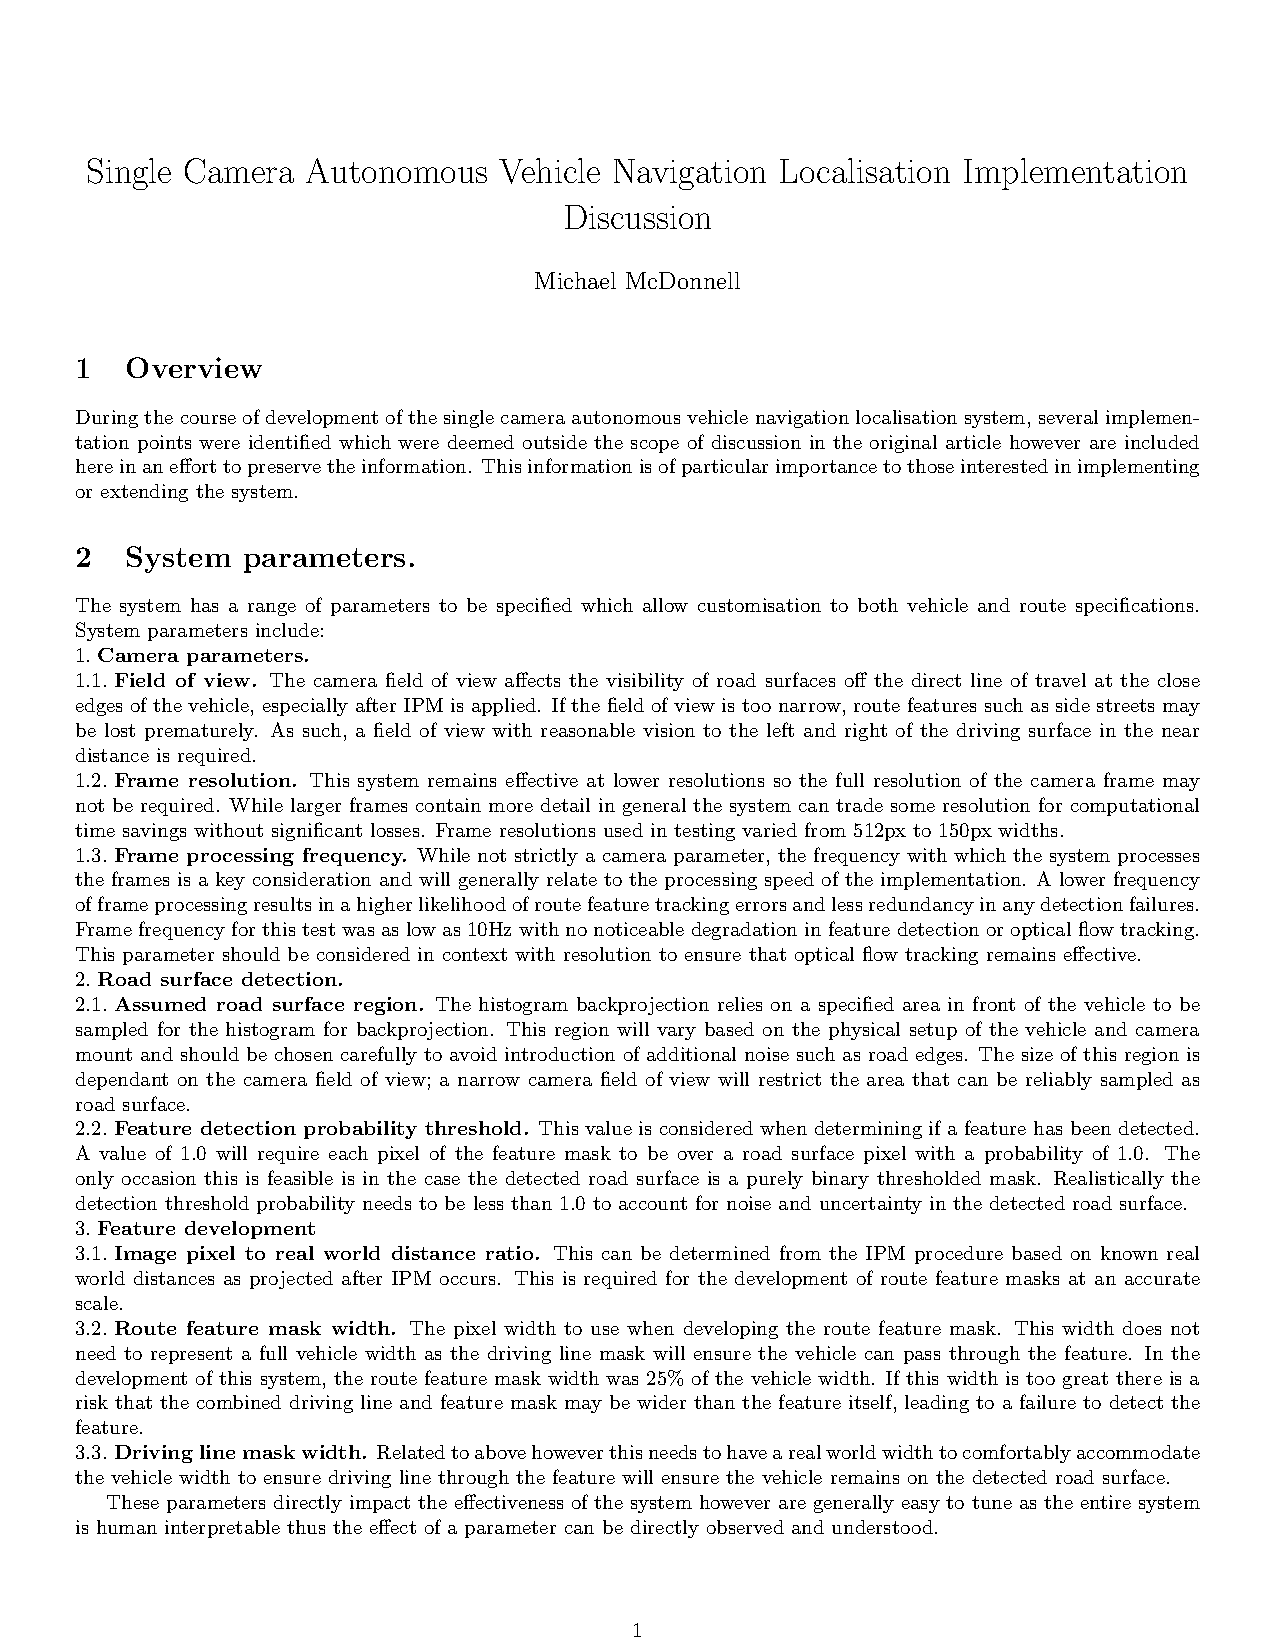
\includepdf[pages=1,scale=.9,pagecommand={\section{Implementation Discussion}\label{app:implementationDiscussion}},linktodoc=false]{implementationDiscussion.pdf}
\includepdf[pages=2-,scale=.9,pagecommand={},linktodoc=false]{implementationDiscussion.pdf}
%\appendix
%\pagestyle{empty}
%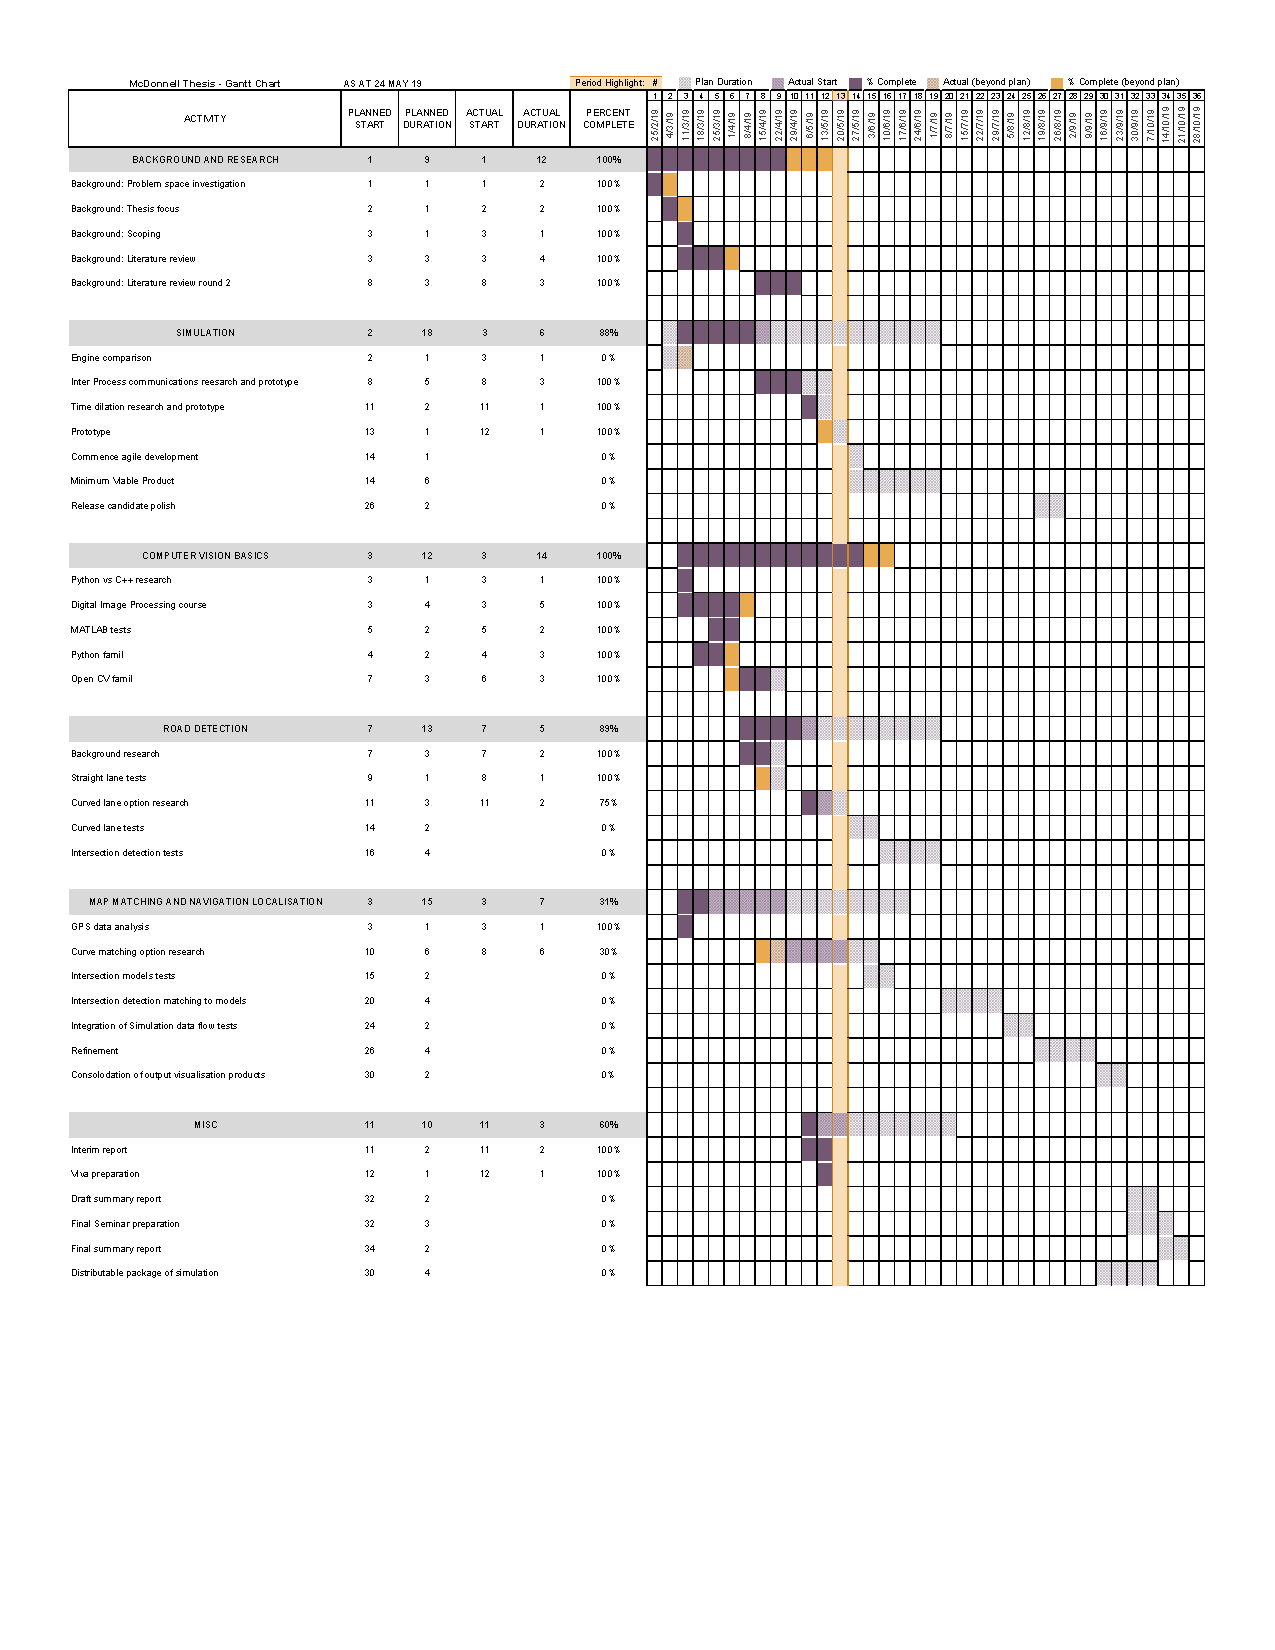
\includepdf[angle=-90,scale=1,pages=1,pagecommand=\section{Gantt Chart for Research Project}\label{app:ganttChart}]{GanttChart.pdf} 

%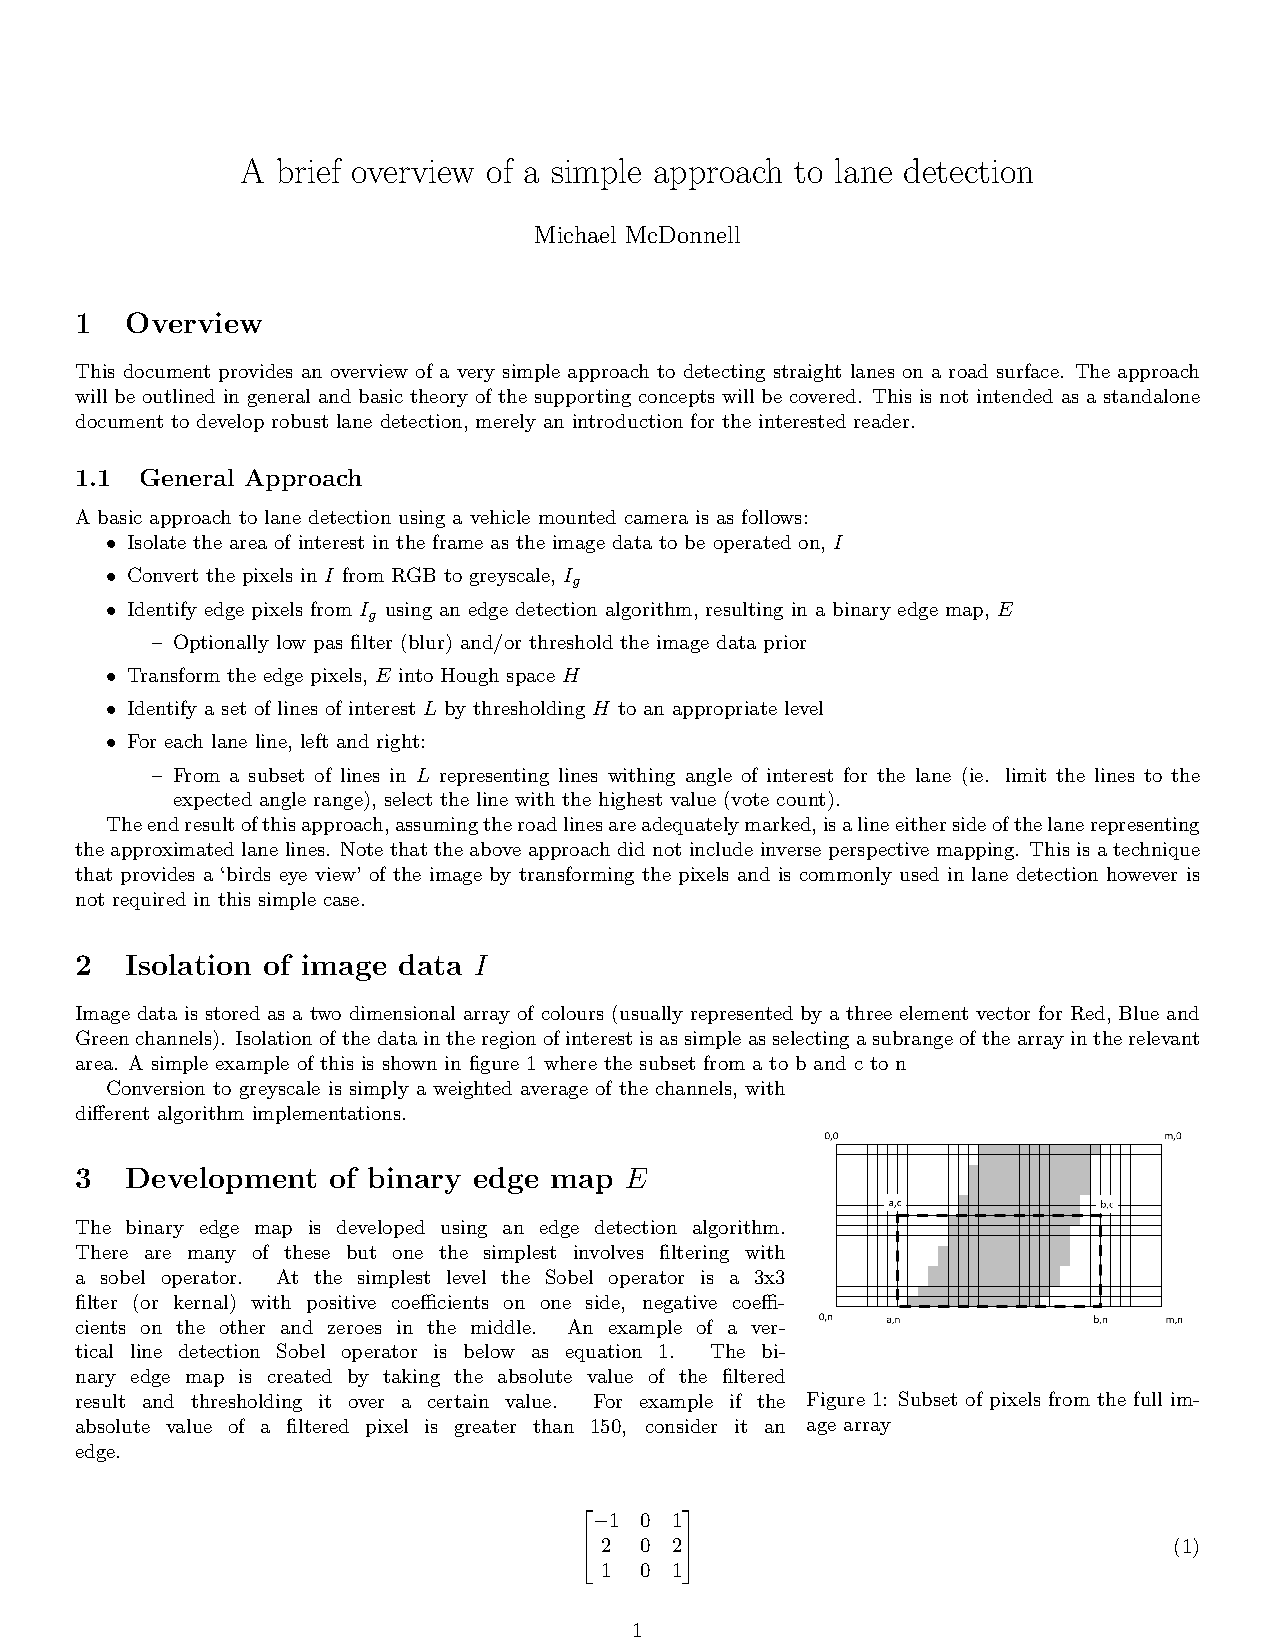
\includepdf[pages=1,scale=.8,pagecommand={\section{A brief overview of a simple approach to lane detection}\label{app:briefOverviewOfLaneDetection}},linktodoc=false]{briefOverviewOfLaneDetection.pdf}
%\includepdf[pages=2-,scale=.8,pagecommand={},linktodoc=false]{briefOverviewOfLaneDetection.pdf}

%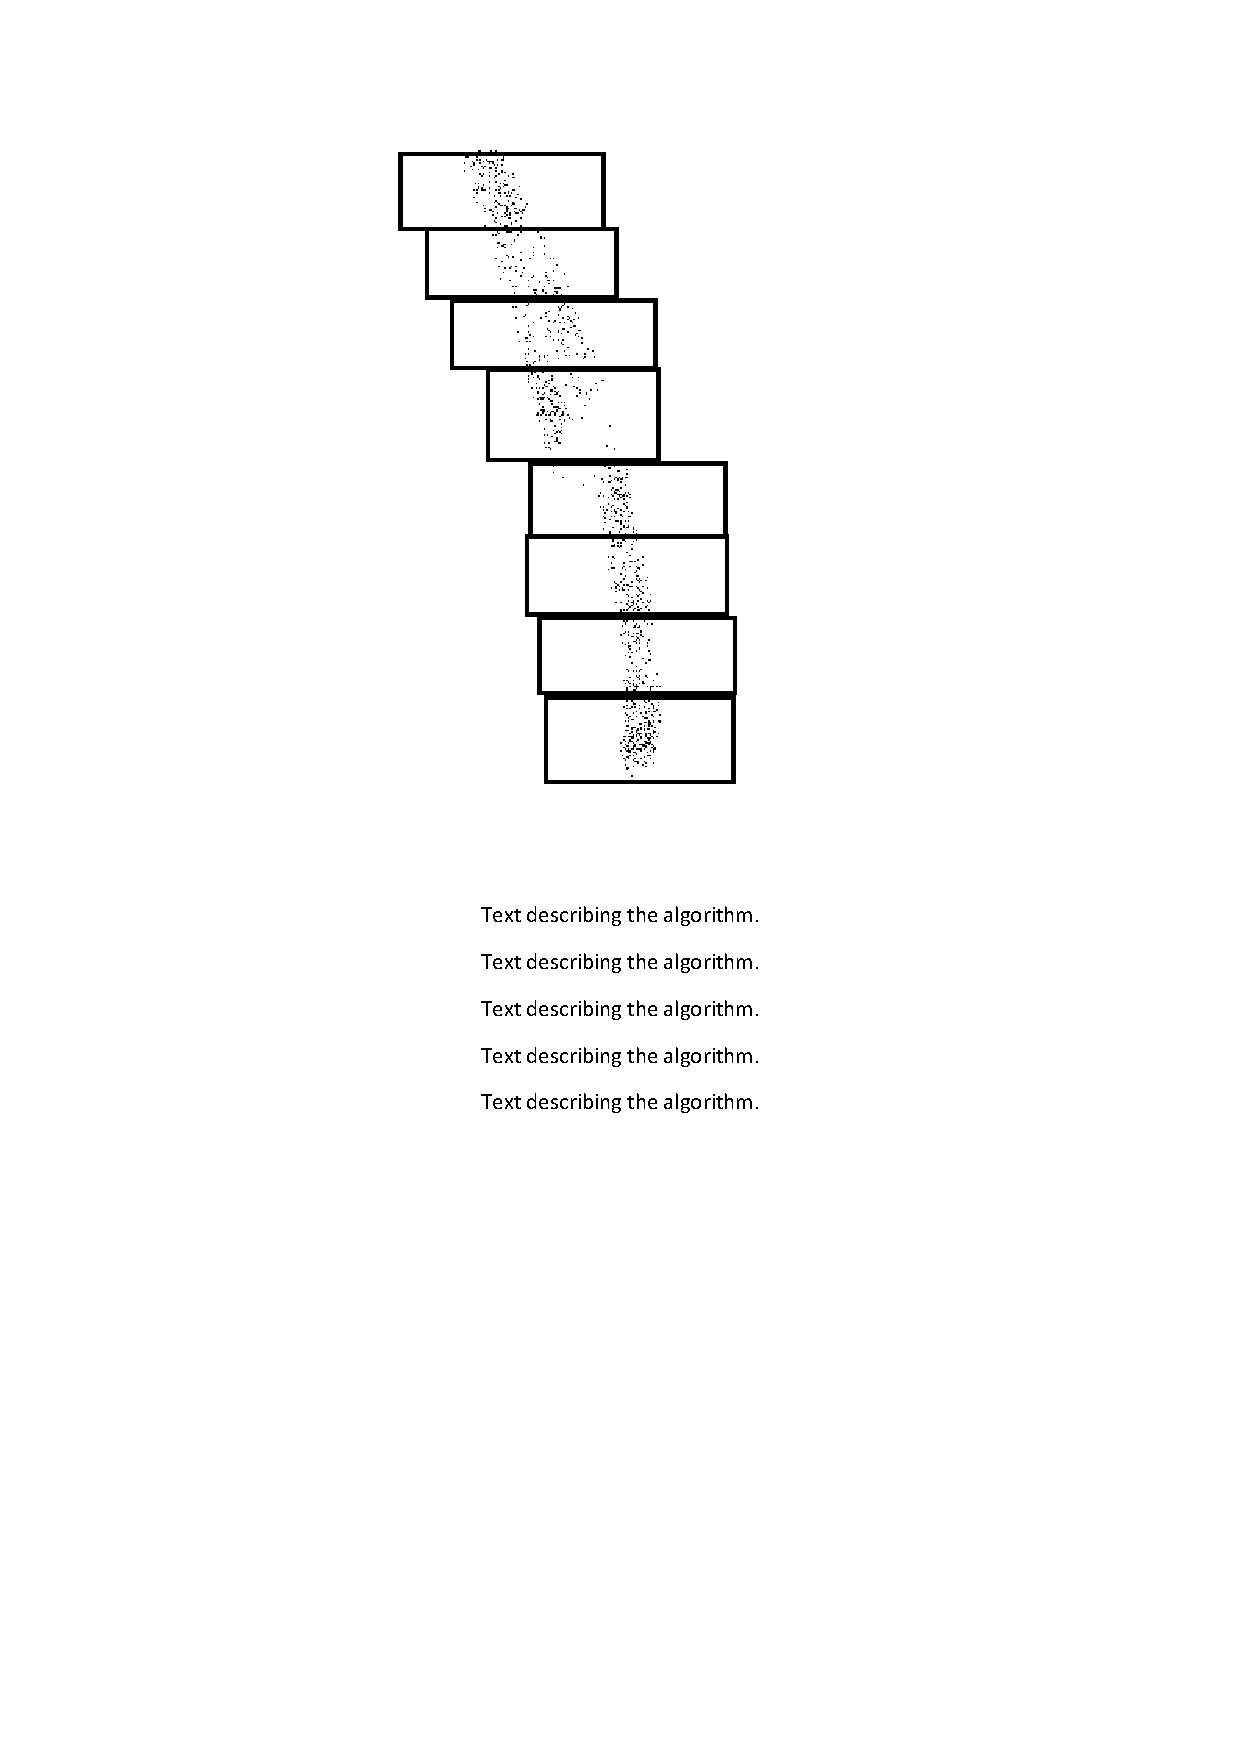
\includepdf[angle=-90,scale=0.9,pages=1,pagecommand=\section{Sliding window detection for curved roads}\label{app:slidingWindow}]{curvedLaneDetection.pdf} 

\end{document}

